\documentclass[conference]{IEEEtran}
\IEEEoverridecommandlockouts
% Add necessary packages here
\usepackage{cite}
\usepackage{amsmath,amssymb,amsfonts}
\usepackage{graphicx}
\usepackage{textcomp}
\usepackage{xcolor}
\usepackage{booktabs}
\usepackage{siunitx}
\usepackage{multirow} % For potentially merging cells in tables
\usepackage{enumitem} % For list customization
\usepackage{url}
\usepackage[colorlinks=false, hidelinks]{hyperref} % Use hidelinks for final print
%--------------------------------------------------------------------

\IEEEoverridecommandlockouts
\IEEEpubid{\makebox[\columnwidth]{979-8-3315-9147-2/25/\$31.00~
\copyright2025
IEEE \hfill} \hspace{\columnsep}\makebox[\columnwidth]{ }}

%--------------------------------------------------------------------

\def\BibTeX{{\rm B\kern-.05em{\sc i\kern-.025em b}\kern-.08em
    T\kern-.1667em\lower.7ex\hbox{E}\kern-.125emX}}

\begin{document}

\makeatletter
\newcommand{\newlineauthors}{%
  \end{@IEEEauthorhalign}\hfill\mbox{}\par
  \mbox{}\hfill\begin{@IEEEauthorhalign}
}
\makeatother

\title{From Assessment to Enhancement of Pull Requests at Scale: Aligning Code Reviews with Developer Competencies Using Large Language Models}

% --- Author Information ---
\author{
\IEEEauthorblockN{Luca Mariotto}
\IEEEauthorblockA{\textit{Mercedes-Benz Tech Innovation}\\
Stuttgart, Germany \\
luca.mariotto@mercedes-benz.com}

\and

\IEEEauthorblockN{Christian Medeiros Adriano}
\IEEEauthorblockA{
\textit{Hasso Plattner Institute}\\
Potsdam, Germany \\
christian.adriano@hpi.de}

\and

\IEEEauthorblockN{René Eichhorn}
\IEEEauthorblockA{
\textit{Mercedes-Benz Tech Innovation}\\
Stuttgart, Germany \\
rene.eichhorn@mercedes-benz.com}

%\and
\newlineauthors

\IEEEauthorblockN{Daniel Burgstahler}
\IEEEauthorblockA{
\textit{Mercedes-Benz Tech Innovation}\\
Stuttgart, Germany \\
daniel.burgstahler@mercedes-benz.com}

\and

\IEEEauthorblockN{Holger Giese}
\IEEEauthorblockA{
\textit{Hasso Plattner Institute}\\
Potsdam, Germany \\
holger.giese@hpi.de}

}

%--------------------

\maketitle
%\IEEEpeerreviewmaketitle

\begin{abstract} 
[Background] Efficient code review is essential in industrial software development, but writing high-quality Pull Request (PR) descriptions aligned with core software engineering competencies remains challenging.
[Aims] To investigate Large Language Models (LLMs) as a reliable PR description assistant, we examined two research problems: (1) how developer competencies relate to real-world PR quality, and (2) how developers perceive PR quality and their variants (LLM-Improved). [Methods] We adopted six software engineering competencies to prompt six LLMs to score 212,687 PRs from 82 open-source projects spanning three repository archetypes. From these, we selected the top six PRs for a controlled experiment with 38 software professionals, using a 6×6 Latin square design to measure preferences. The LLMs generated three variants of each original (O) PR: degraded (D), improved from the original (IO), and improved from the degraded (ID). We then compared these variants across LLMs for semantic, lexical, and stylistic similarity. [Results] Surprisingly, our controlled experiment with 38 software professionals showed that the ID variant was rated significantly higher than both the Original PR (O) and the LLM-Degraded (D) one. However, the IO variant was not significantly better, and participants complained about their verbosity and the "AI tone". Concerning generalizability, the six LLMs produced semantically similar PRs, but with high lexical and stylistic variation. [Conclusions] This suggests LLMs can enhance PR by providing missing structure but require guidance to retain human nuance. Overall, our findings support human-centered, model-aware integration of LLMs to strengthen competency-aligned code review.
\end{abstract}

\begin{IEEEkeywords}
Code Review, Pull Requests, Automated Quality Assessment, Software Metrics, and Empirical Study.
\end{IEEEkeywords}

\section*{Lay Abstract}

[Background] Efficient code review is essential in industrial software development, but it isn't easy to assess Pull Request (PR) quality at scale and align it with reviewer competencies. [Aims] We investigated: (1) how developer competencies relate to real-world PR quality, and (2) how developers perceive PR quality variants (LLM-Improved). [Methods] We used six competencies to guide six LLMs in scoring 212,687 PRs from 82 open-source repositories of various types. We selected six high-quality PRs from these and prompted the LLMs to produce improved and degraded versions of their descriptions. Professional programmers compared and scored these LLM-generated versions. [Results] Surprisingly, participants rated the LLM-Improved degraded (ID) variant significantly higher than both the original (O) and degraded (D) versions. However, they criticized the improved original (IO) variants for their verbosity and an overly "AI-like" tone. While the six LLMs produced semantically similar PRs, their lexical and stylistic outputs varied widely.  [Conclusions] LLMs can enhance PR clarity and structure, but require human-centered, model-aware integration to preserve nuance and support competency-aligned code reviews.

\section{Introduction} 
Industrial software development demands high quality and rapid delivery cycles, making efficient code review essential \cite{mcintosh2014impact}. Because most code reviews nowadays happen in the context of Pull Requests (PR), a bottleneck for the software team, particularly when PRs are incomplete or inconsistent with the code change~\cite{bacchelli2013expectations}. PRs produced by junior programmers or project newcomers tend to be more problematic~\cite{khatoonabadi2023wasted,kovalenko2018code
}.

While Large Language Models (LLM) have shown benefits to assist developers in understanding and generating code~\cite{fan2023large,cui2025effects}, this is unclear for code review. To translate the potential of LLMs into a valuable and reliable code review assistant in an industrial setting, we investigate two sets of practical research problems: (1) how developer's competencies relate to real-world PR quality, and (2) how developers perceive original PR quality and their variants (LLM-Improved). The first research problem is partitioned into the following research questions:
\begin{itemize}
    \item \textbf{RQ1:} Can automated, competency-based scoring provide meaningful insights into PR quality across diverse projects at scale, supporting process monitoring or improvement efforts?
    \item \textbf{RQ2:} How consistent are different LLMs performing the same SE assistance task? Understanding model agnosticism is vital for tool selection, maintenance, and ensuring a predictable user experience.
\end{itemize}

To tackle these questions, we conducted large-scale automated quality scoring on 212,687 PRs from 82 diverse open-source repositories using zero-shot classification based on six code review engineering competencies\cite{wurzel2023competencies}. This analysis uncovered distinct quality profiles and project archetypes, demonstrating the feasibility of scalable, automated PR evaluation.
To evaluate model agnosticism, we tested six state-of-the-art LLMs (ChatGPT-4o, Claude Sonnet, Deepseek Deepthink, Gemini Flash, Grok, Qwen) by generating and comparing controlled PR description variants (Degraded, Improved).
Results showed partial semantic consistency (SBERT cosine=0.74, BERTScore F1=0.85), but significant variability in lexical and stylistic features (BLEU=0.03), highlighting limitations in consistency and user experience when switching between models. Our findings support the importance of model-aware tool design to manage variability, cost, and user trust.

We address the second research problem by partitioning it in two research questions:
\begin{itemize}
    \item \textbf{RQ3:} How do developers perceive the relative quality of original human-written (O), LLM-degraded (D), LLM-improved from degraded (ID), and LLM-improved from original (IO) PR descriptions?
    \item \textbf{RQ4:} What specific factors (e.g., structure, detail, conciseness, tone, perceived source) drive these perceptions?
\end{itemize}

To answer these two last questions, we conducted a controlled experiment with 38 software professionals assessing LLM-generated PR descriptions. Participants compared Original (O) human-written descriptions with Degraded (D), Improved from Original (IO), and Improved from Degraded (ID) versions produced through a multi-stage LLM pipeline. Surprisingly, the ID variants were rated significantly higher than both D (p-value=0.029) and O (p-value=0.026), mainly due to the added structure and clarity introduced by the models. However, IO variants were not statistically significant preferred (p-value$>$0.05) and often received negative feedback for verbosity and a generic "AI tone". These results suggest that LLMs can enhance clarity and structure but must be guided carefully to avoid output homogenization and loss of human-authored nuance.

This research was partly conducted with Mercedes-Benz Tech Innovation GmbH, and our contributions comprise: 
\begin{enumerate}
    \item Large-scale automated PR scoring based on SE competencies \cite{wurzel2023competencies}; 
    \item A quantitative evaluation comparing outputs of six modern LLMs generating PR description variations. Automated scoring reveals project archetypes, and LLMs exhibit partial model agnosticism – semantic intent transfers, but crucial stylistic characteristics vary significantly, impacting practical deployment.
    \item The sets of scripts, dataset, and LLM prompts are publicly available for reproducibility and further investigations\footnote{\url{https://github.com/LucaMariotto/llm-code-review-thesis-artifacts/}. The scripts referenced in this paper are indexed in the file \textit{Scripts-Index-Table.pdf}}. Similarly, the LLM prompts and corresponding data can be found in the \textit{prompts} and \textit{data} folders, respectively.
\end{enumerate}

\textbf{Paper tour} --  Section-\ref{sec:background} introduces key concepts, followed by Section-\ref{sec:sota} on recent advances and research gaps. Methodology and results are covered in Sections IV to VII for RQ1–RQ4. Section-\ref{sec:implications} discusses industry implications, Section-\ref{sec:discussion_limitations} addresses limitations, and Section-\ref{sec:conclusion} concludes with contributions and future work.

%----------------------------

\section{Background}\label{sec:background}

\subsection{Code Review}
Code review is the systematic inspection of the source code by individuals other than the original author with the goals of: defect detection early in the life-cycle~\cite{bavota2015four}, improving code quality (i.e., readability, maintainability, and adherence to standards)~\cite{gousios2015work}, knowledge sharing for  the onboarding of newcomers and creating learning opportunities for junior developers~\cite{bacchelli2013expectations, bosu2013building}. 

\subsection{Pull Requests}
In contemporary distributed software development, particularly when using version control systems like Git, code review is most commonly facilitated through the Pull Request (PR) mechanism (also known as Merge Requests in platforms like GitLab). The PR workflow provides a structured process for proposing, discussing, and integrating code changes \cite{gousios2015work}.

A typical PR workflow involves the following steps:
\begin{enumerate}
    \item A developer makes changes to the codebase in a separate branch.
    \item The developer creates a Pull Request, signaling their intent to merge these changes into a target branch (often the main development branch).
    \item The PR includes the proposed code changes (the "diff") and, crucially, a description provided by the author. This description typically explains the purpose of the changes, the problem being solved, the approach taken, and potentially provides instructions for reviewers or links to relevant issue trackers.
    \item Assigned or interested reviewers examine the code changes and the description.
    \item Reviewers provide feedback through comments directly on the PR, potentially suggesting modifications, asking questions, or approving the changes.
    \item A discussion ensues between the author and reviewers, often involving iterations where the author addresses feedback by pushing further code changes to the PR branch.
    \item Once the reviewers are satisfied and any required automated checks (e.g., \textit{linters} and continuous integration tests) pass, the PR is finally approved and merged into the target branch.
\end{enumerate}

The \textbf{Pull Request description} plays a pivotal role in this workflow. A well-written description significantly aids reviewers by providing essential context, clarifying the rationale behind the changes, and guiding their attention to critical areas. It helps reviewers understand the "why" behind the "what" (the code changes), making the review process more efficient and effective \cite{gousios2014exploratory}. Conversely, a poor or missing description can force reviewers to spend considerable extra time reverse-engineering the author's intent, increasing review latency and potentially leading to superficial reviews \cite{kononenko2015investigating}. The quality and content of PR descriptions are thus critical for the smooth functioning of the review process.

\subsection{Code Review Competence}\label{sec:competence} 
To evaluate the PRs and prompt the LLM to produce personalized versions of these PRs, we adopted a set of six competencies, as discussed in \cite{wurzel2023competencies}:
\begin{enumerate}
 \item \textbf{Architecture Impact:} \label{comp:architecture} Evaluates architectural implications and design pattern changes.

    \item \textbf{Code Quality:} \label{comp:codequality} Assesses code correctness, error handling, and technical debt.

    \item \textbf{Collaboration:} \label{comp:collaboration} Evaluates communication clarity and team collaboration aspects.

    \item \textbf{Maintainability:} \label{comp:maintainability} Analyzes documentation, modularity, and long-term viability.

    \item \textbf{User Impact:} \label{comp:userimpact} Assesses user-facing changes and UX considerations.

    \item \textbf{Technical Leadership:} \label{comp:techleadership} Measures influence on technical direction and mentoring.
    \end{enumerate}

\subsection{Similarity Metrics}\label{sec:similarity-metrics}

In the model agnosticism evaluation, we adopted various metrics to compare the PR content:
\begin{itemize}
    \item \textbf{Lexical Similarity:} Metrics that measure overlap based on exact words or sequences (n-grams) - BLEU\cite{papineni2002bleu} and ROUGE-L~\cite{lin2004rouge} -longest common subsequences. Low scores indicate differences in phrasing and word choice.
    \item \textbf{Semantic Similarity:} Metrics that measure overlap based on meaning, often using text embeddings, such as SBERT Cosine Similarity~\cite{papineni2002bleu} and BERTScore~\cite{zhang2020bertscore}. High scores indicate that the core meaning is preserved even if the wording differs.
    \item \textbf{Term-Based Similarity:} Metrics that measure overlap based on important terms (keywords), such as TF-IDF Cosine Similarity.
\end{itemize}


%--------------------------------------

\section{The State-of-the-Art}\label{sec:sota}
\textbf{Pull request quality} can be evaluated using established metrics \cite{li2003ranking} and a range of code review competencies. These competencies encompass technical aspects such as code quality, architectural impact, and human-centered concerns, including collaboration, maintainability, user impact, and technical leadership \cite{wurzel2023competencies}. Ensuring software quality increasingly depends on techniques like defect prediction \cite{zhang2022machine} and automated program repair \cite{huang2024evolving}. In parallel, advances in automated task partitioning \cite{adriano2016exploring,latoza2014microtask} and newcomer onboarding \cite{tan2025revolutionizing,steinmacher2018let} have empowered large-scale developer participation in both code contributions \cite{aghayi2023controlled} and bug inspection tasks \cite{adriano2022microtasking}. Adopting large language models (LLMs) aligns with these ongoing trends in automating software engineering tasks and supporting human-in-the-loop workflows. However, the large-scale, multi-dimensional scoring of review competencies and personalization of pull request (PR) textual content—explored in this work—represents a relatively novel direction.

\textbf{Model agnosticism }is a practical concern for deploying LLMs in industry ~\cite{devireddy2025comparative}. Although techniques exist to address this ~\cite{wang2024natural, horne2023vader}, there is a lack of comparative studies that measure output traits—such as length, style, and readability—across modern LLMs for tasks like PR enhancement. Our study fills this gap by comparing semantic consistency and stylistic variation, both critical for industrial adoption.

\textbf{AI/ML support} has advanced from reviewer recommendation \cite{thongtanunam2015should, zanjani2016automatically} to using Deep Learning and LLMs for tasks like generating comments or suggesting fixes \cite{tufano2022using, li2022automating, froemmgen2024resolving, lu2023llama}. However, reliability issues like hallucinations \cite{tonmoy2024comprehensive}, lack of robustness \cite{li2025enhancing}, and poor instruction following \cite{wang2025codeif} persist.  Meanwhile, effective review requires diverse human competencies \cite{wurzel2023competencies}, including social skills, which AI struggles to replicate \cite{yang2024survey}. For these reasons, AI-based tools must integrate human factors and promote trust in their capabilities \cite{mehrotra2024systematic,kim2023humans}. We aim to improve AI tool design by integrating LLMs into the PR workflow and evaluating the quality of PR variants.

\textbf{Current limitations} Recent work emphasizes LLM limitations in alignment and controllability, often producing homogenized outputs that lack authenticity \cite{lee2025poor}, which can negatively impact perceived quality. Personalization~\cite{zhang2024personalization} and nudging~\cite{maddila2023nudge,caraban2019ways} have been explored in prior work. However, systematic evaluation of perceived quality for core artifacts like PR descriptions—especially in terms of structure versus style—remains limited. Our work directly addresses this perceptual gap.

\section{Methodology for RQ1 and RQ2}
\subsection{Automated PR Quality Scoring}
\subsubsection{Data Collection and Preparation}
We fetched 212,687 PRs (created Jan 2022 - Apr 2025) from 82 diverse, popular open-source GitHub repositories using the GraphQL API (script \texttt{S1}). Repositories spanned domains like Web Frameworks (e.g., `rails/rails`, `django/django`), Databases (`postgres/postgres`, `redis/redis`), ML/AI (`pytorch/pytorch`, `tensorflow/tensorflow`), Languages (`golang/go`, `rust-lang/rust`), OS (`torvalds/linux`, `systemd/systemd`), and DevOps (`ansible/ansible`, `grafana/grafana`). We filtered PRs to retain those with 5-15 comments (inclusive) to focus on substantive but manageable discussions, yielding a dataset for scoring (script \texttt{D2}).

\subsubsection{Scoring Process}
Using script \texttt{S2}, the textual content (title, body, comments) of each filtered PR was scored using a zero-shot classification pipeline\footnote{\texttt{MoritzLaurer/ModernBERT-large-zeroshot-v2.0}\cite{warner2024smarter}.}. This model predicts the likelihood that the text pertains to predefined labels without specific training. The output score (0-1) represents the classifier's confidence for each code review competency label (Sec.\ref{sec:competence}).

\subsubsection{Analysis}
We computed descriptive statistics (mean, standard deviation, script \texttt{S8}) for all PR scores, aggregated results for 77 repositories with over 10 analyzed PRs (script \texttt{D3}). We examined score variation across repositories using Kruskal-Wallis tests and assessed inter-competency correlations via Spearman rho at both PR and repository levels. We identified archetypes with PCA and K-Means clustering (K=3) on standardized repository mean scores (scripts \texttt{D4,D8}).

\subsection{Model Agnosticism Evaluation}
We developed a support tool that automatically extracts PRs, processes them via LLM prompting, and allows two experts to compare two PRs side-by-side (\ref{fig:activity-diagram-tool}).

\begin{figure}[htbp]
    \centering
    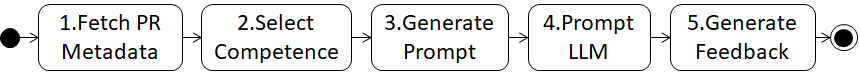
\includegraphics[width=\linewidth]{evaluation/images/activity_diagram_PR-Competence-Prompt.png} 
    \caption{Tool based on GitHub Action workflow for delivering personalized LLM-based feedback.}
    \label{fig:activity-diagram-tool}
\end{figure}

\subsubsection{Setup}
We used six baseline PRs (O) selected via scoring and dual-expert validation (rated 'good' by both experts). For each O, we generated three variations using competency-guided prompts:
\begin{itemize}[noitemsep, topsep=0pt]
    \item \textbf{Degraded (D):} Prompted to reduce quality aspects (e.g., clarity, detail).
    \item \textbf{Improved Original (IO):} Prompted to enhance O based on competencies.
    \item \textbf{Improved Degraded (ID):} Prompted to enhance D based on competencies.
\end{itemize}
This was performed using six LLMs:
\begin{itemize}[noitemsep, topsep=0pt]
    \item \textbf{Baseline}: ChatGPT-4o-latest (reasoning)
    \item \textbf{Alternatives}: Claude 3.7 Sonnet, Deepseek Deepthink R1 (thinking), Gemini 2.0 Flash (thinking), Grok 3 (thinking), Qwen2.5-Max (thinking QwQ)
\end{itemize}

\subsubsection{Comparison Metrics}
\begin{itemize}[noitemsep, topsep=0pt]
    \item \textbf{Text Quality Metrics:} Word/sentence counts, Flesch Reading Ease (higher=easier), Flesch-Kincaid Grade Level (lower=simpler)\cite{kincaid1975}, Sentiment (NLTK VADER compound score -1 to +1)\cite{hutto2014vader}. These metrics were calculated for each generated version (script \texttt{D11}).
    \item \textbf{Similarity Metrics (vs. Baseline):} (script \texttt{D7})
        \begin{itemize}[noitemsep]
        \item \textit{Lexical:} BLEU (n-gram precision, 0-1), ROUGE-L F1 (longest common subsequence, 0-1).
        \item \textit{Semantic:} SBERT Cosine Similarity (embedding similarity, -1 to +1), BERTScore F1 (contextual embedding overlap, 0-1).
        \end{itemize}
\end{itemize}
We analyzed descriptive statistics and performed pairwise statistical tests (Mann-Whitney U with Bonferroni correction) on readability metrics (script \texttt{D10}).

\section{Answers to RQ1 and RQ2}
\subsection{Automated Scoring Findings}
\begin{itemize}
    \item \textbf{Overall Scores:} Across 212k+ PRs, mean scores varied by competency (e.g., Collaboration: 0.45, Tech. Leadership: 0.24). Std dev also varied (Code Quality: 0.32, Tech. Leadership: 0.24).
    \item \textbf{Repository Variation:} Significant differences in mean competence score were identified between repositories (Kruskal-Wallis $p_{corr} < 0.001$ (see Fig. \ref{fig:repo_score_distributions_igc_enriched}).
    \item \textbf{Correlations:} Nonetheless, the competency correlations were generally weak at the repository level (Fig.\ref{fig:competency_correlation_igc_enriched}), e.g., $\rho=0.39$ (Arch. vs User Impact). Similar weak patterns were observed at the PR level.
    \item \textbf{Repository Archetype:} K-Means clustering (K=3) on repository means yielded distinct profiles, Fig.\ref{fig:kmeans_clusters_pca_igc_enriched}; Table.\ref{tab:cluster_summary}:
        \begin{itemize}[noitemsep, topsep=0pt]
        \item Cluster 0 (N=40): High Architectural, Technical, and User Impact; Low Collaboration. Medium volume.
        \item Cluster 1 (N=27): High Code Quality and Collaboration.; Low Architectural Decisions and Maintainability. High volume.
        \item Cluster 2 (N=10): High Maintainability; Low Code Quality and User Impact. Highest volume.
        \end{itemize}
    This suggests that automated scoring can capture differing quality focuses at scale. (script \texttt{D12}).
\end{itemize}

\begin{figure}[htbp] % Existing Figure
    \centering
    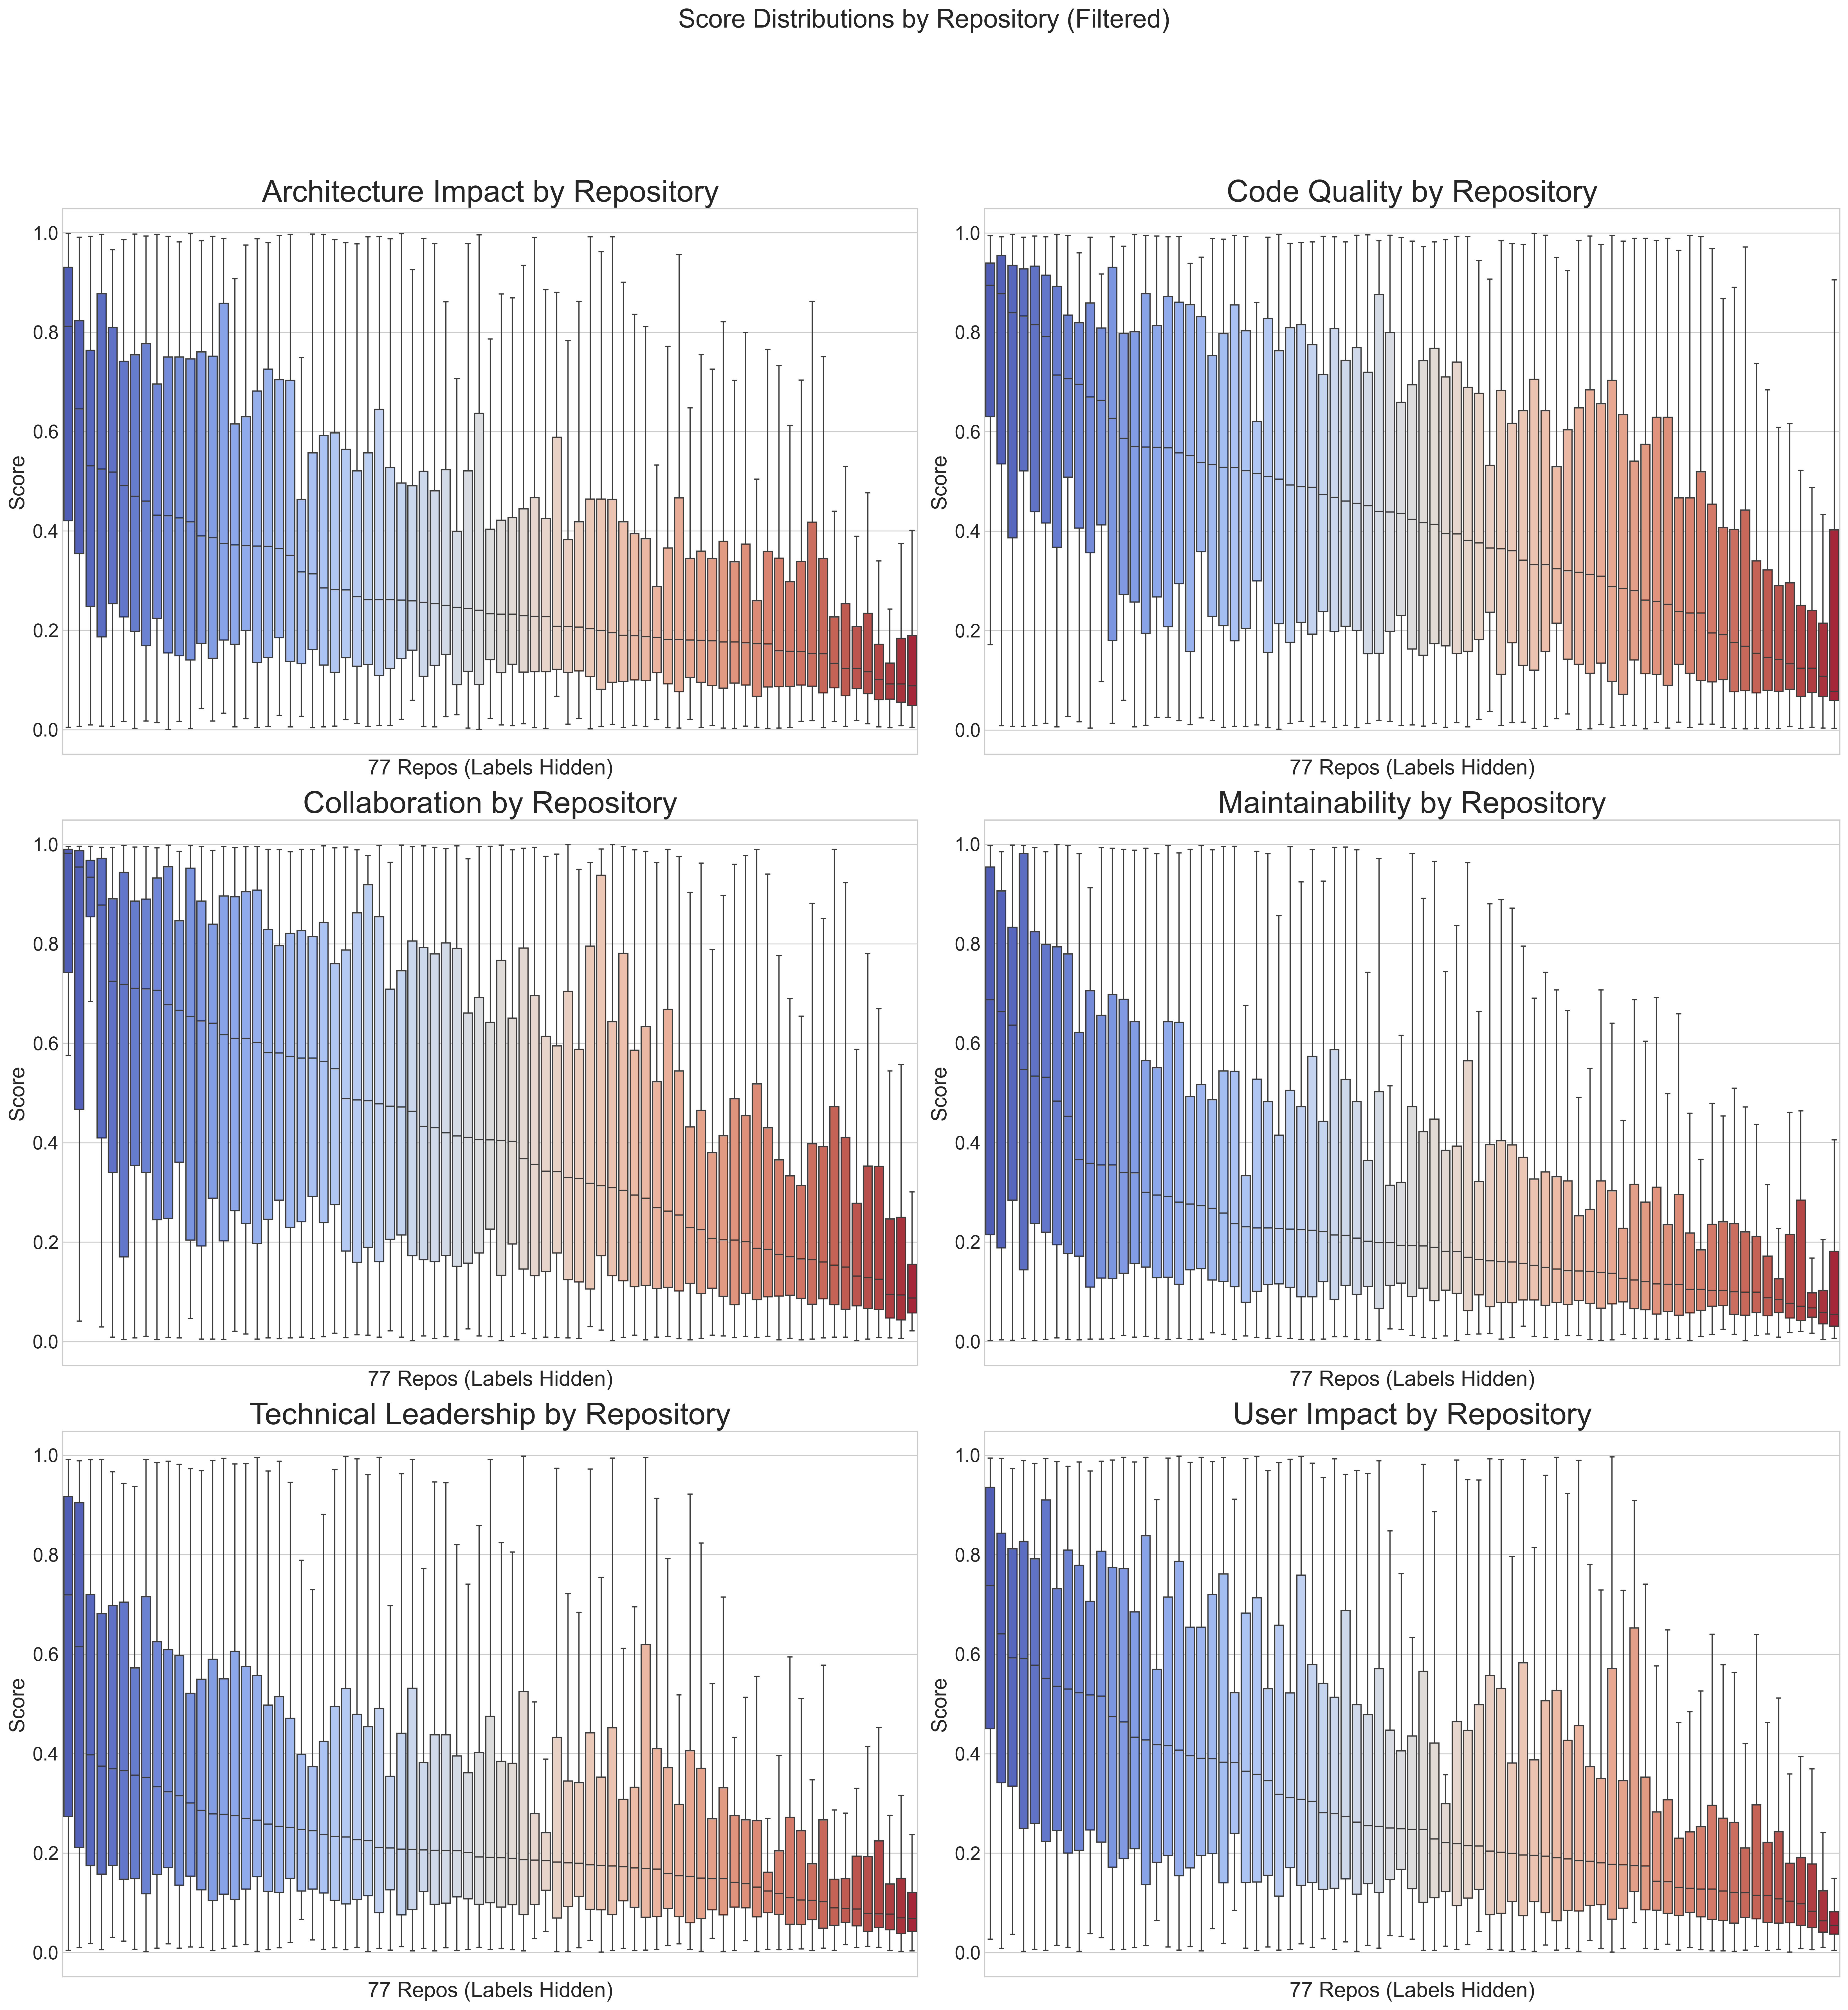
\includegraphics[width=\linewidth]{evaluation/images/repo_score_distributions_bundled.png} % Replace with actual path
    \caption{Distribution of Mean Competency Scores across Repositories.}
    \label{fig:repo_score_distributions_igc_enriched}
\end{figure}

\begin{figure}[htbp] % Existing Figure
    \centering
    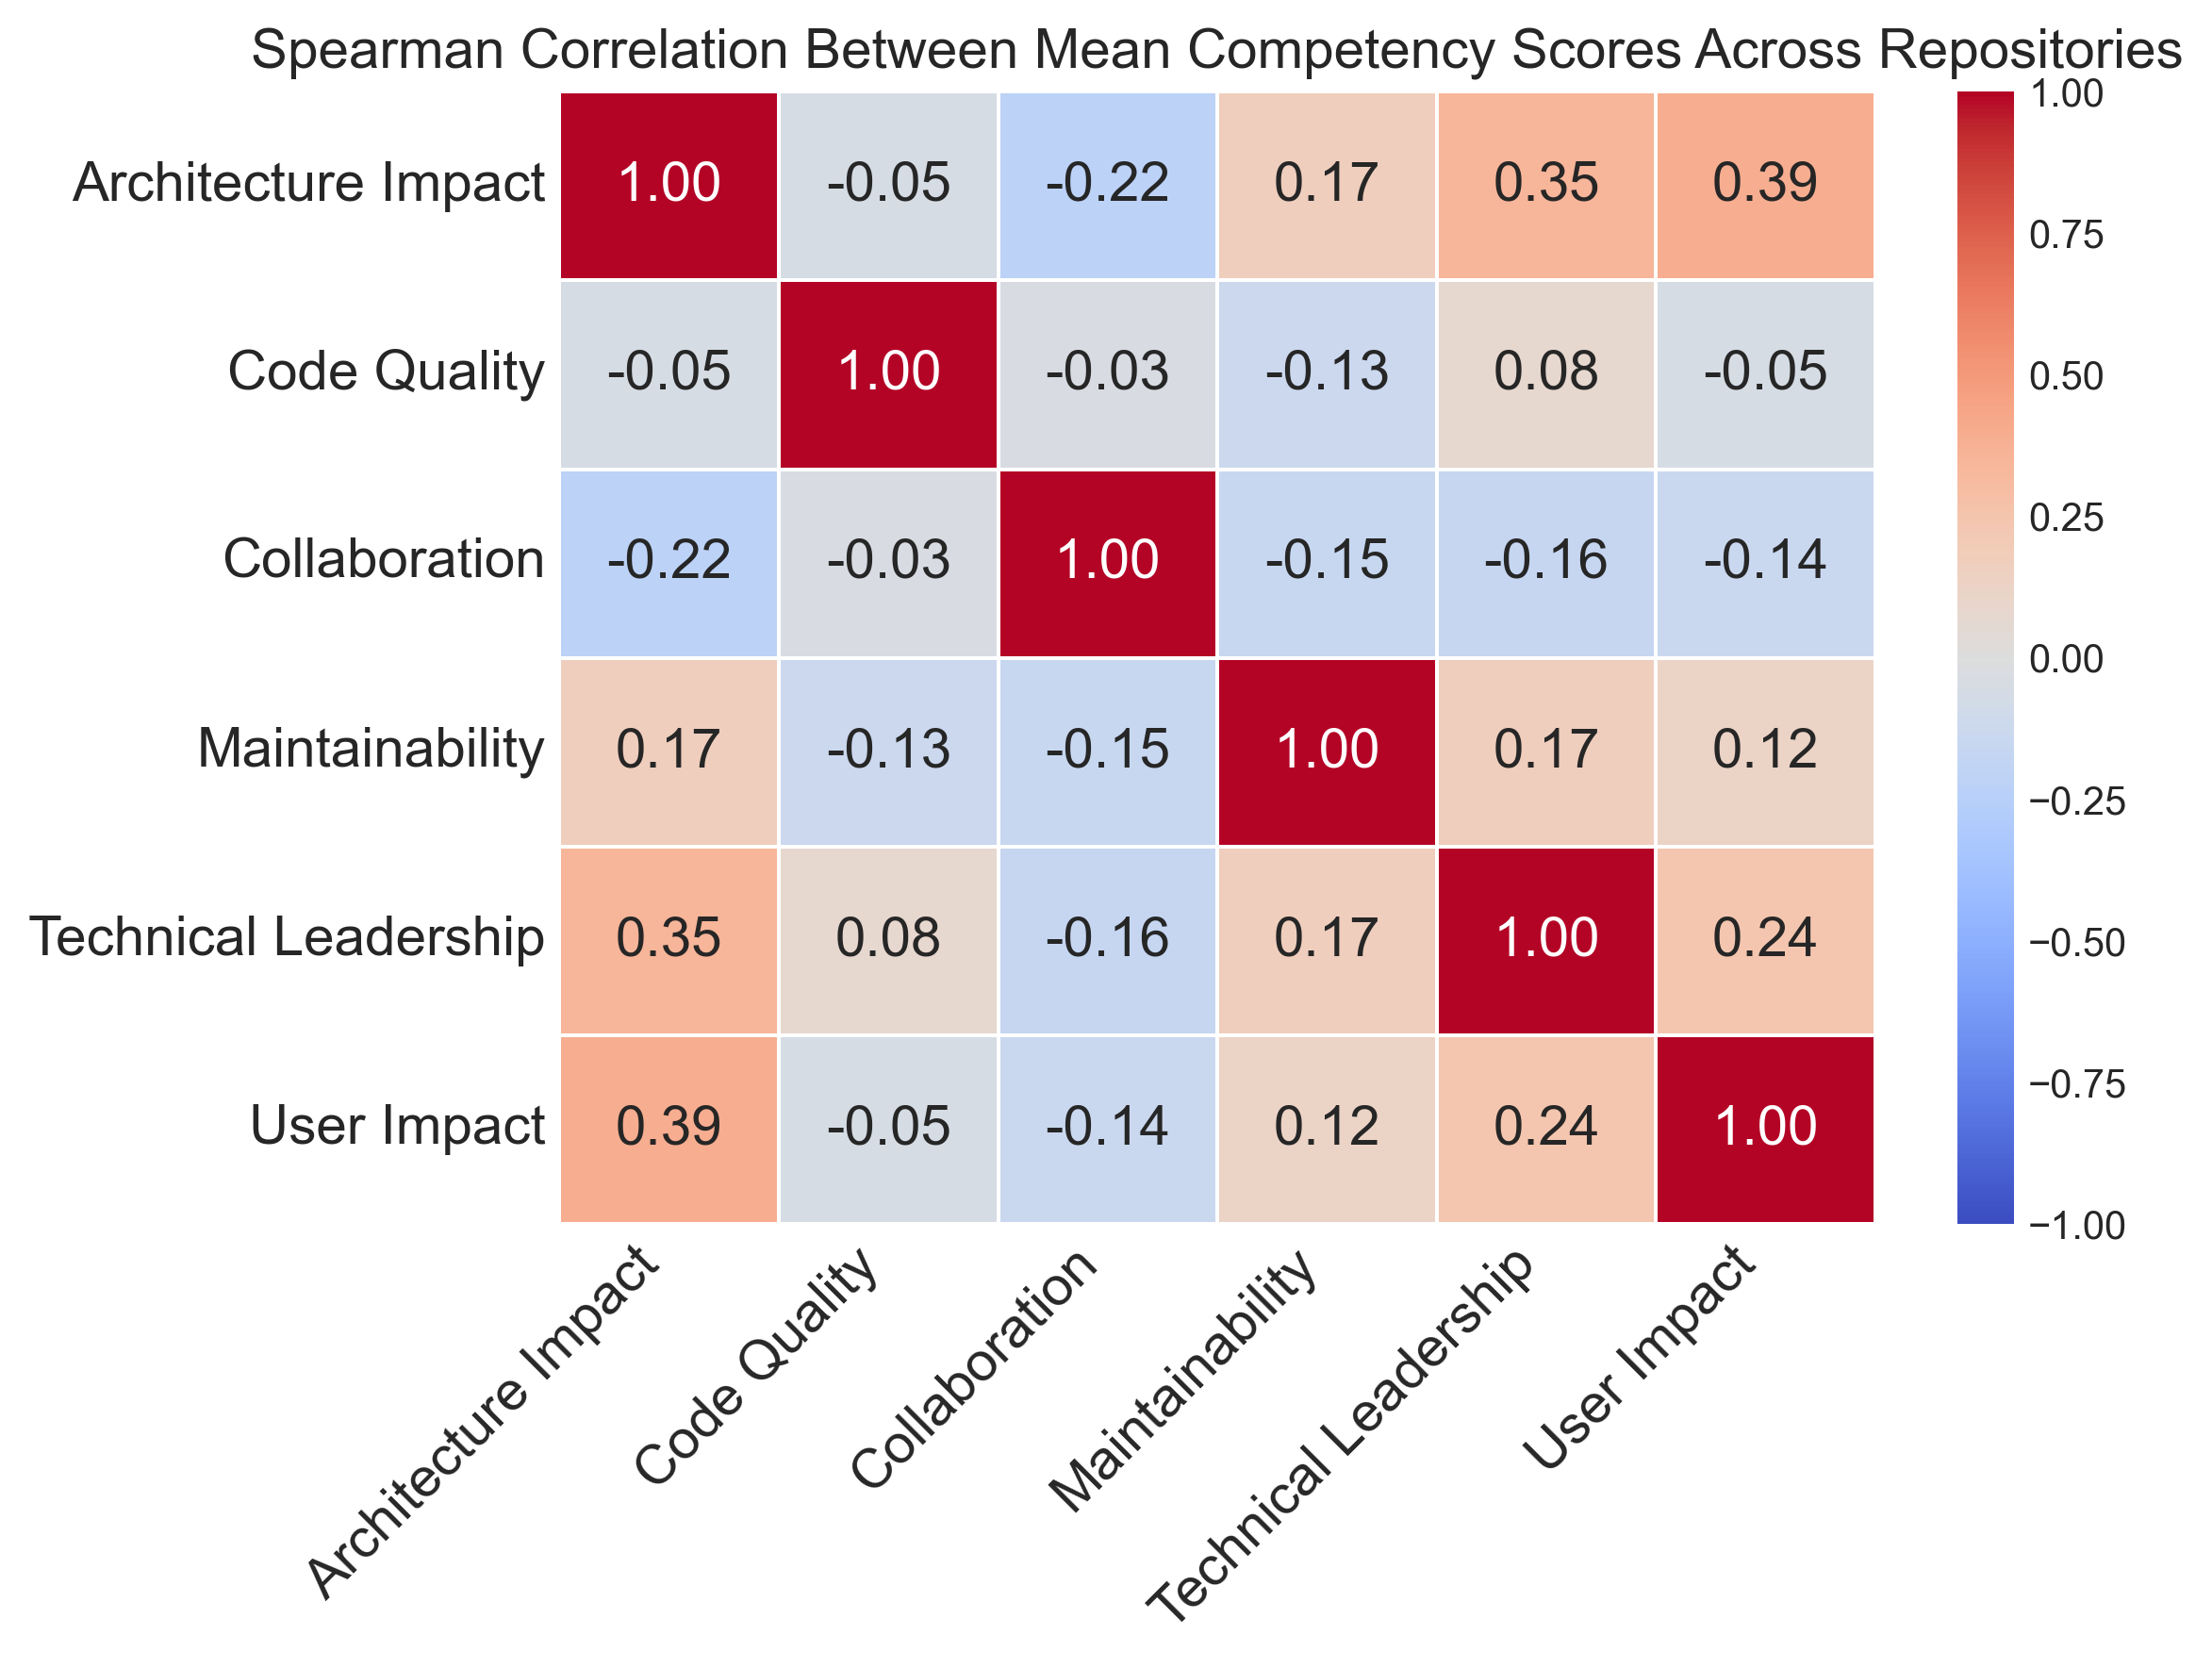
\includegraphics[width=0.7\linewidth]{evaluation/images/competency_correlation_heatmap.png} % Replace with actual path
    \caption{Repository-Level Mean Competency Score Correlations.}
    \label{fig:competency_correlation_igc_enriched}
\end{figure}

\begin{figure}[htbp] % Existing Figure
    \centering
     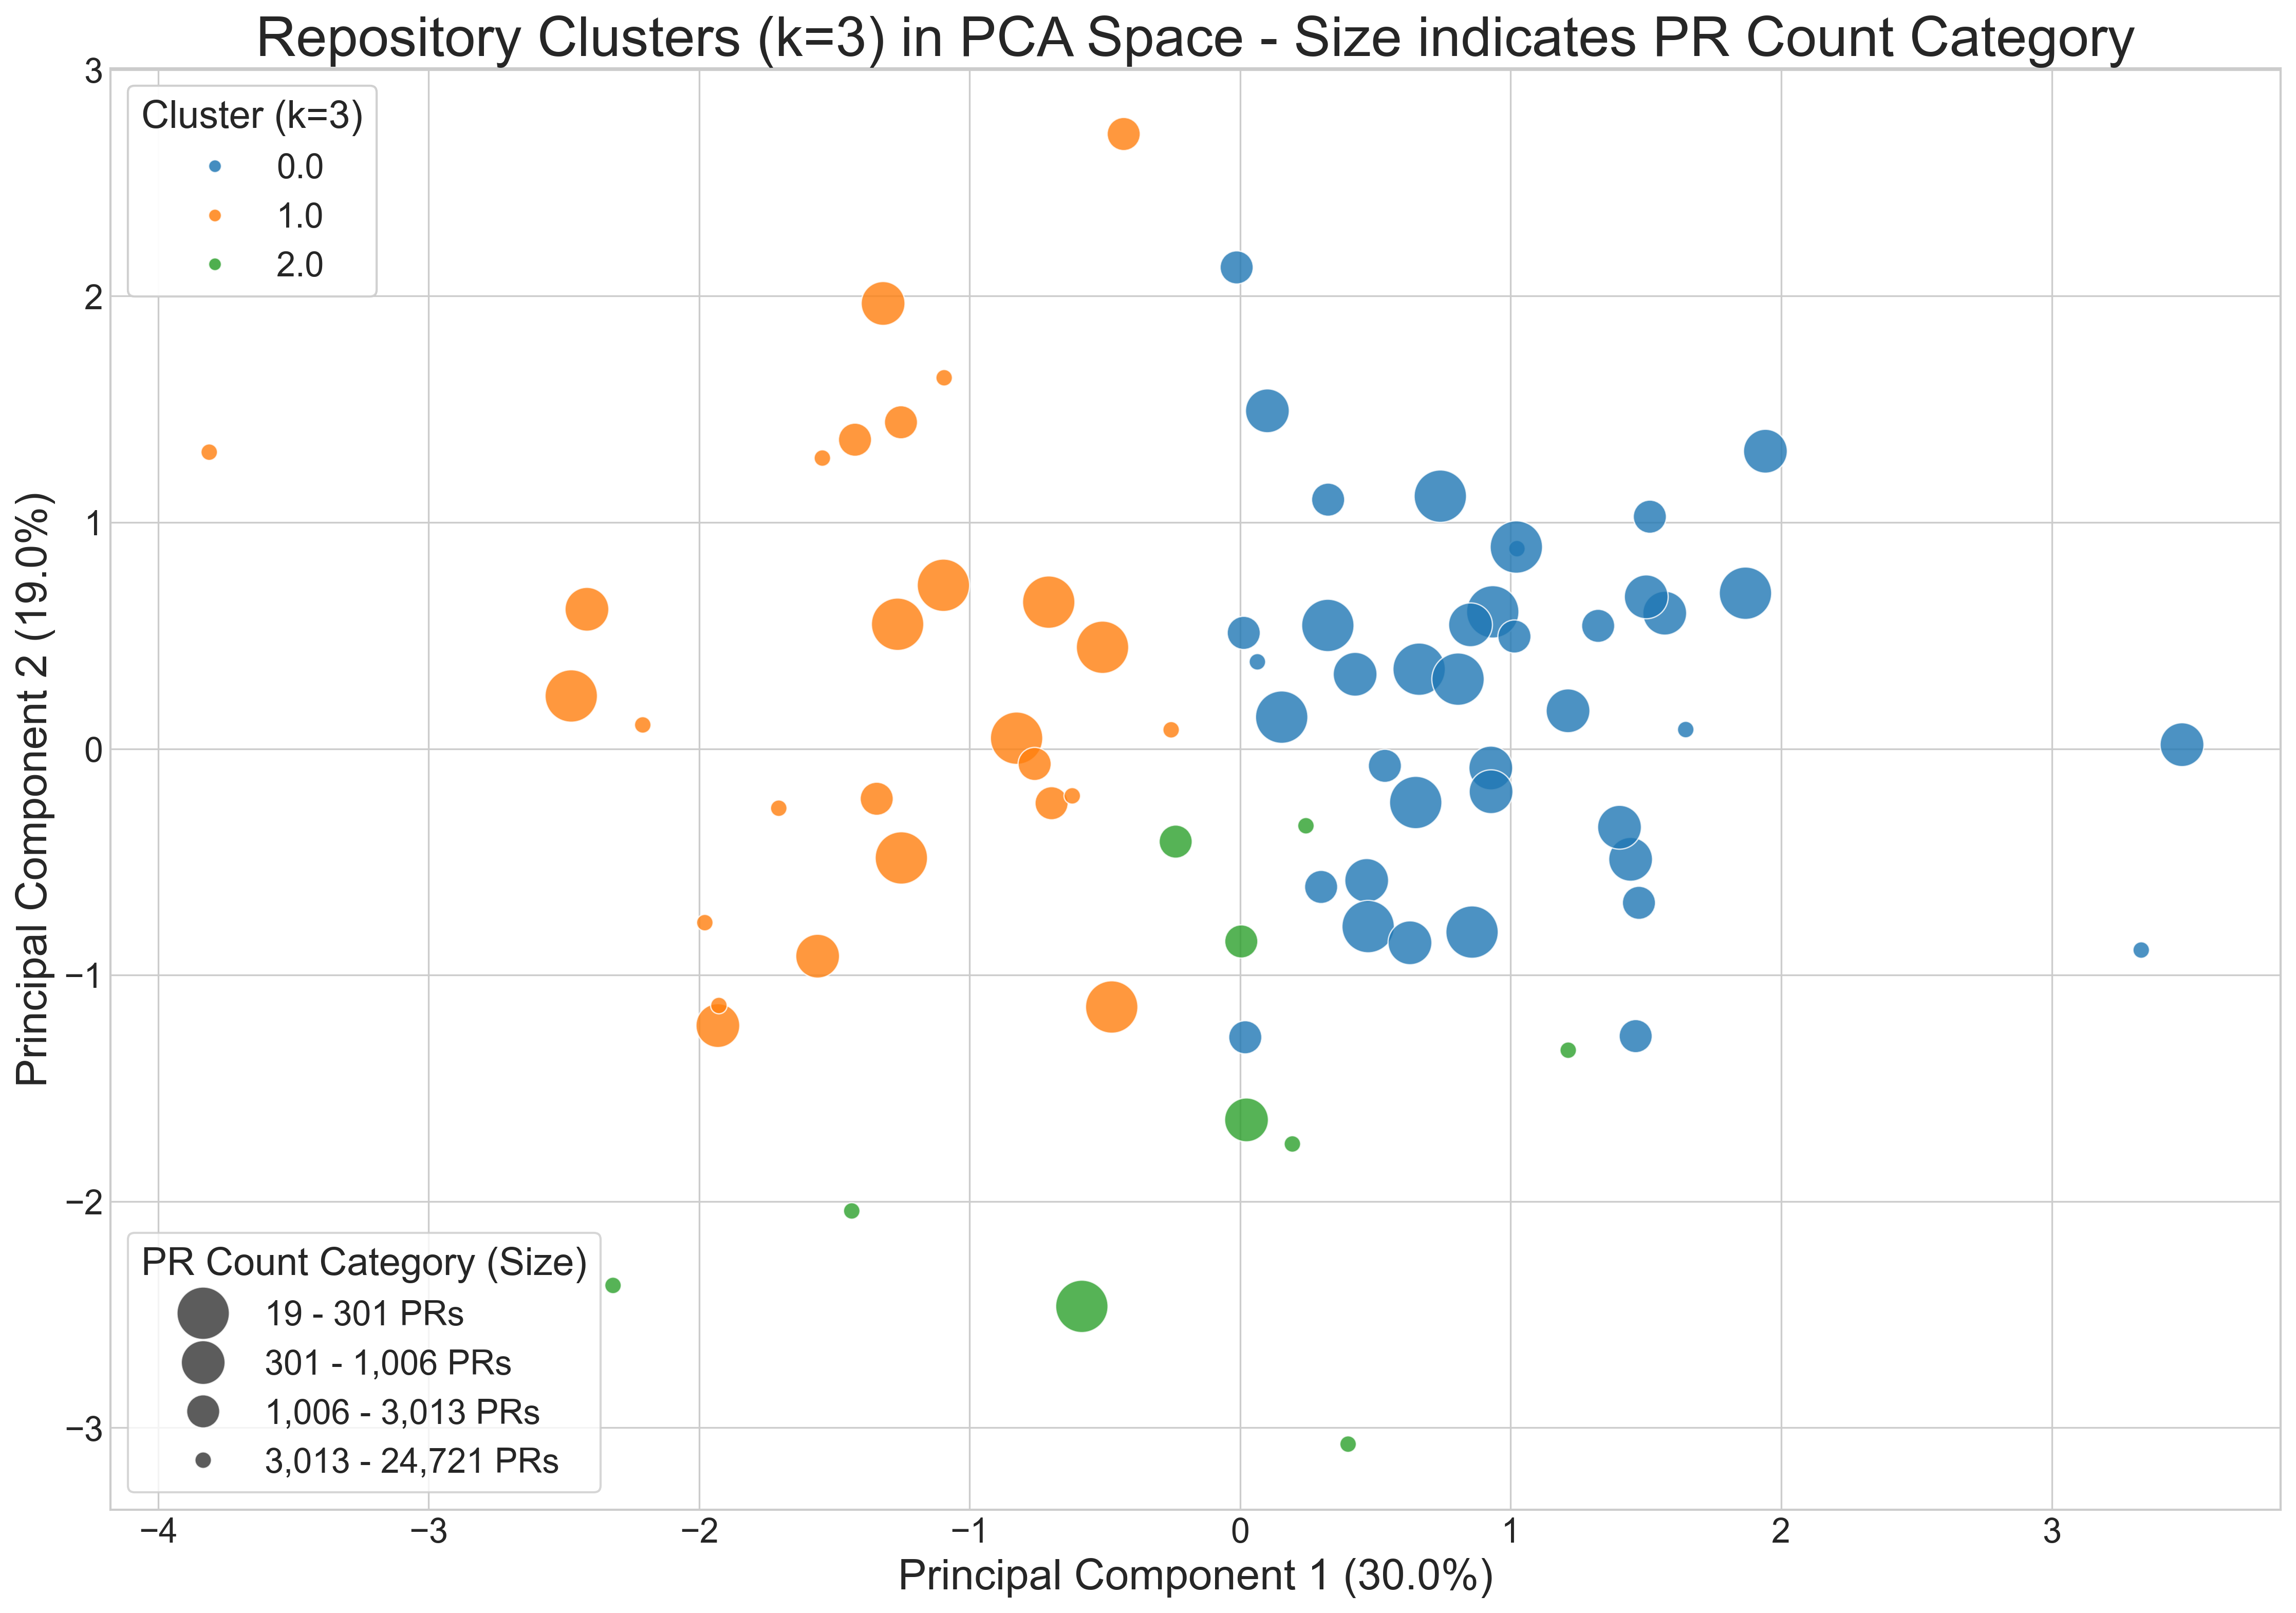
\includegraphics[width=0.8\linewidth]{evaluation/images/kmeans_clusters_pca_binned_size.png} % Replace with actual path
    \caption{K-Means Clusters of Repositories (PCA Projection).}
    \label{fig:kmeans_clusters_pca_igc_enriched}
\end{figure}

% Add Cluster Summary Table
\begin{table}[htbp]
\centering
\caption{Mean Competency Scores per Repository Cluster (K=3)}
\label{tab:cluster_summary}
\sisetup{round-mode=places, round-precision=2}
\resizebox{\linewidth}{!}{% Resize table to fit column width
\begin{tabular}{l S S S}
\toprule
Competency          & {Cluster 0 (N=40)} & {Cluster 1 (N=27)} & {Cluster 2 (N=10)} \\
\midrule
Architecture Impact & 0.40 & 0.19 & 0.24 \\
Code Quality        & 0.43 & 0.50 & 0.37 \\
Collaboration       & 0.36 & 0.52 & 0.46 \\
Maintainability     & 0.23 & 0.28 & 0.47 \\
User Impact         & 0.40 & 0.25 & 0.22 \\
Technical Leadership& 0.34 & 0.18 & 0.21 \\
\midrule
Median PR Count     & {793} & {1814} & {3720} \\
\bottomrule
\end{tabular}%
}
\end{table}

The average classifier confidence falls within [0-1] (see TABLE \ref{tab:cluster_summary}).

%---------------------------------------------------

\subsection{Model Agnosticism Findings}
\subsubsection{Metric Variability}
Directional impacts held (Fig. \ref{fig:agnosticism_readability_by_version_igc_enriched}): 'Improved' versions (ID/IO) were significantly more complex to read (lower Flesch Ease) than D ($p < 1.14 \times 10^{-6}$), reflecting added complexity. Absolute word count values varied greatly by LLM, e.g., IO ranged from 422 (Deepseek) to 1744 (Claude) (Fig. \ref{fig:agnosticism_word_count_by_llm_igc_enriched}). Table \ref{tab:agnosticism_metrics_summary} shows variability for IO versions.

\begin{figure}[htbp] % Existing Figure
    \centering
    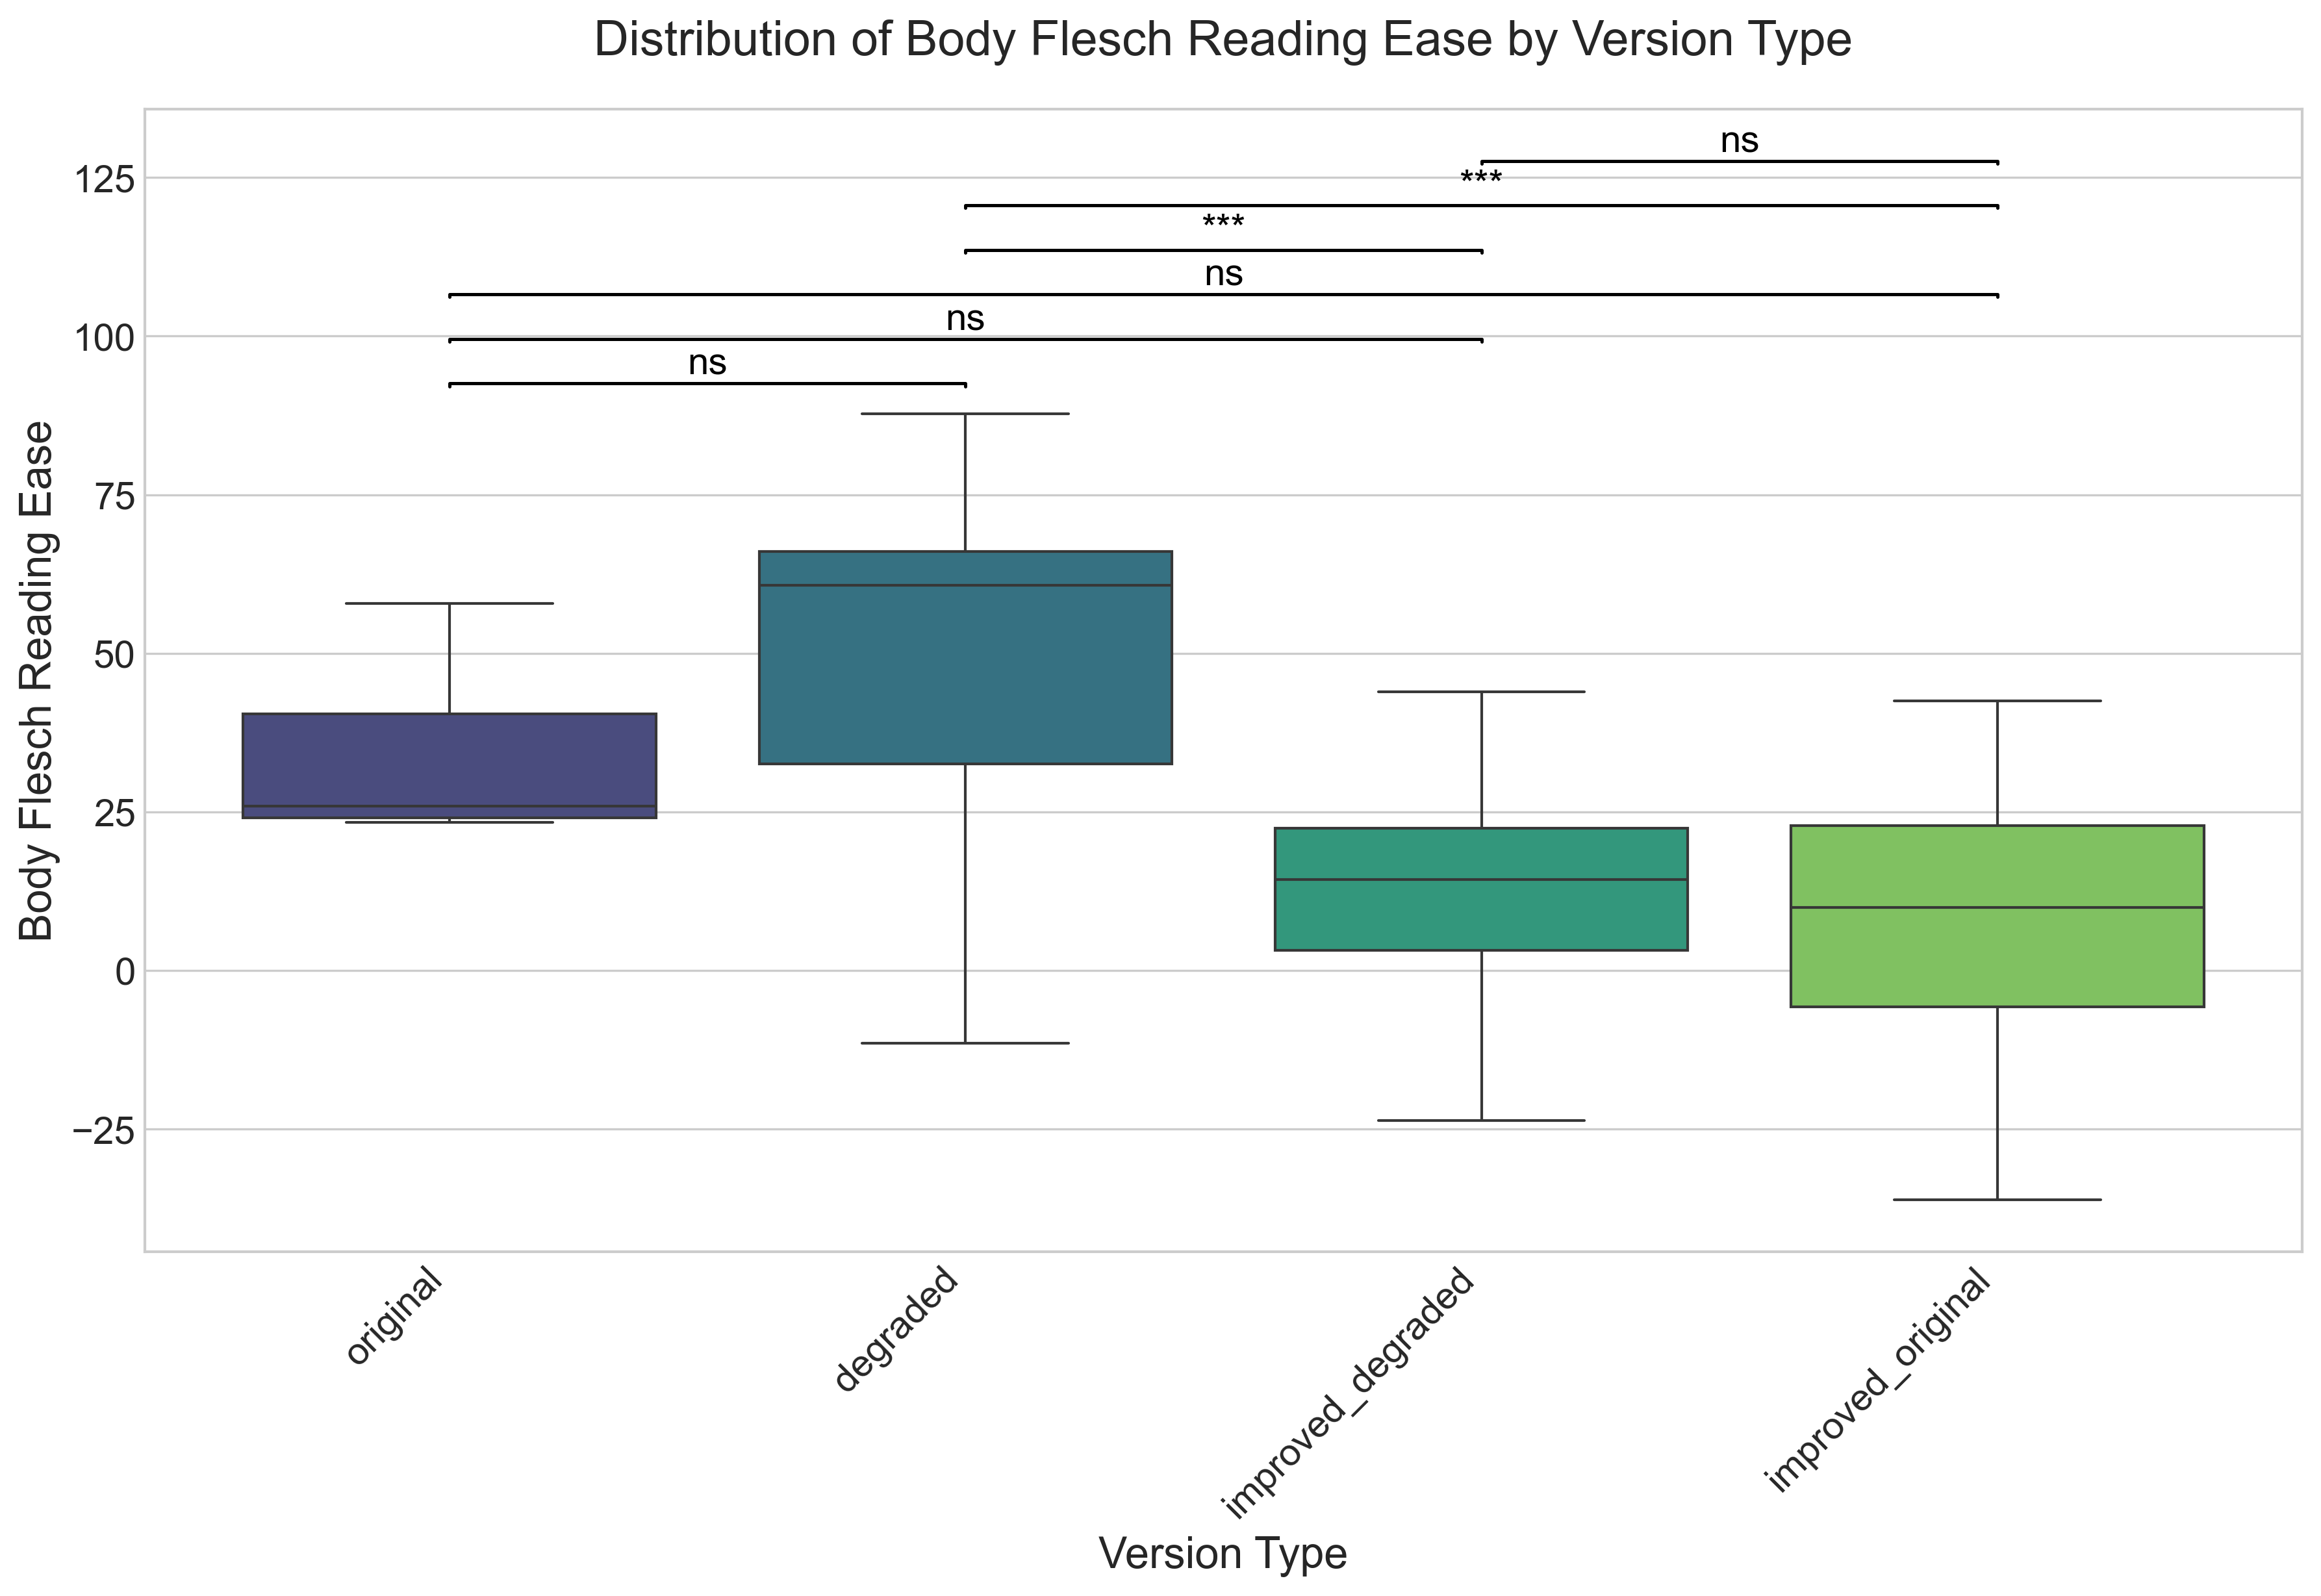
\includegraphics[width=0.8\linewidth]{evaluation/images/variability_by_version_body_readability_flesch_reading_ease.png} % Replace with actual path
    \caption{Average Flesch Reading Ease (Body Text) by Version Type.}
    \label{fig:agnosticism_readability_by_version_igc_enriched}
\end{figure}

\begin{figure}[htbp] % Existing Figure
    \centering
    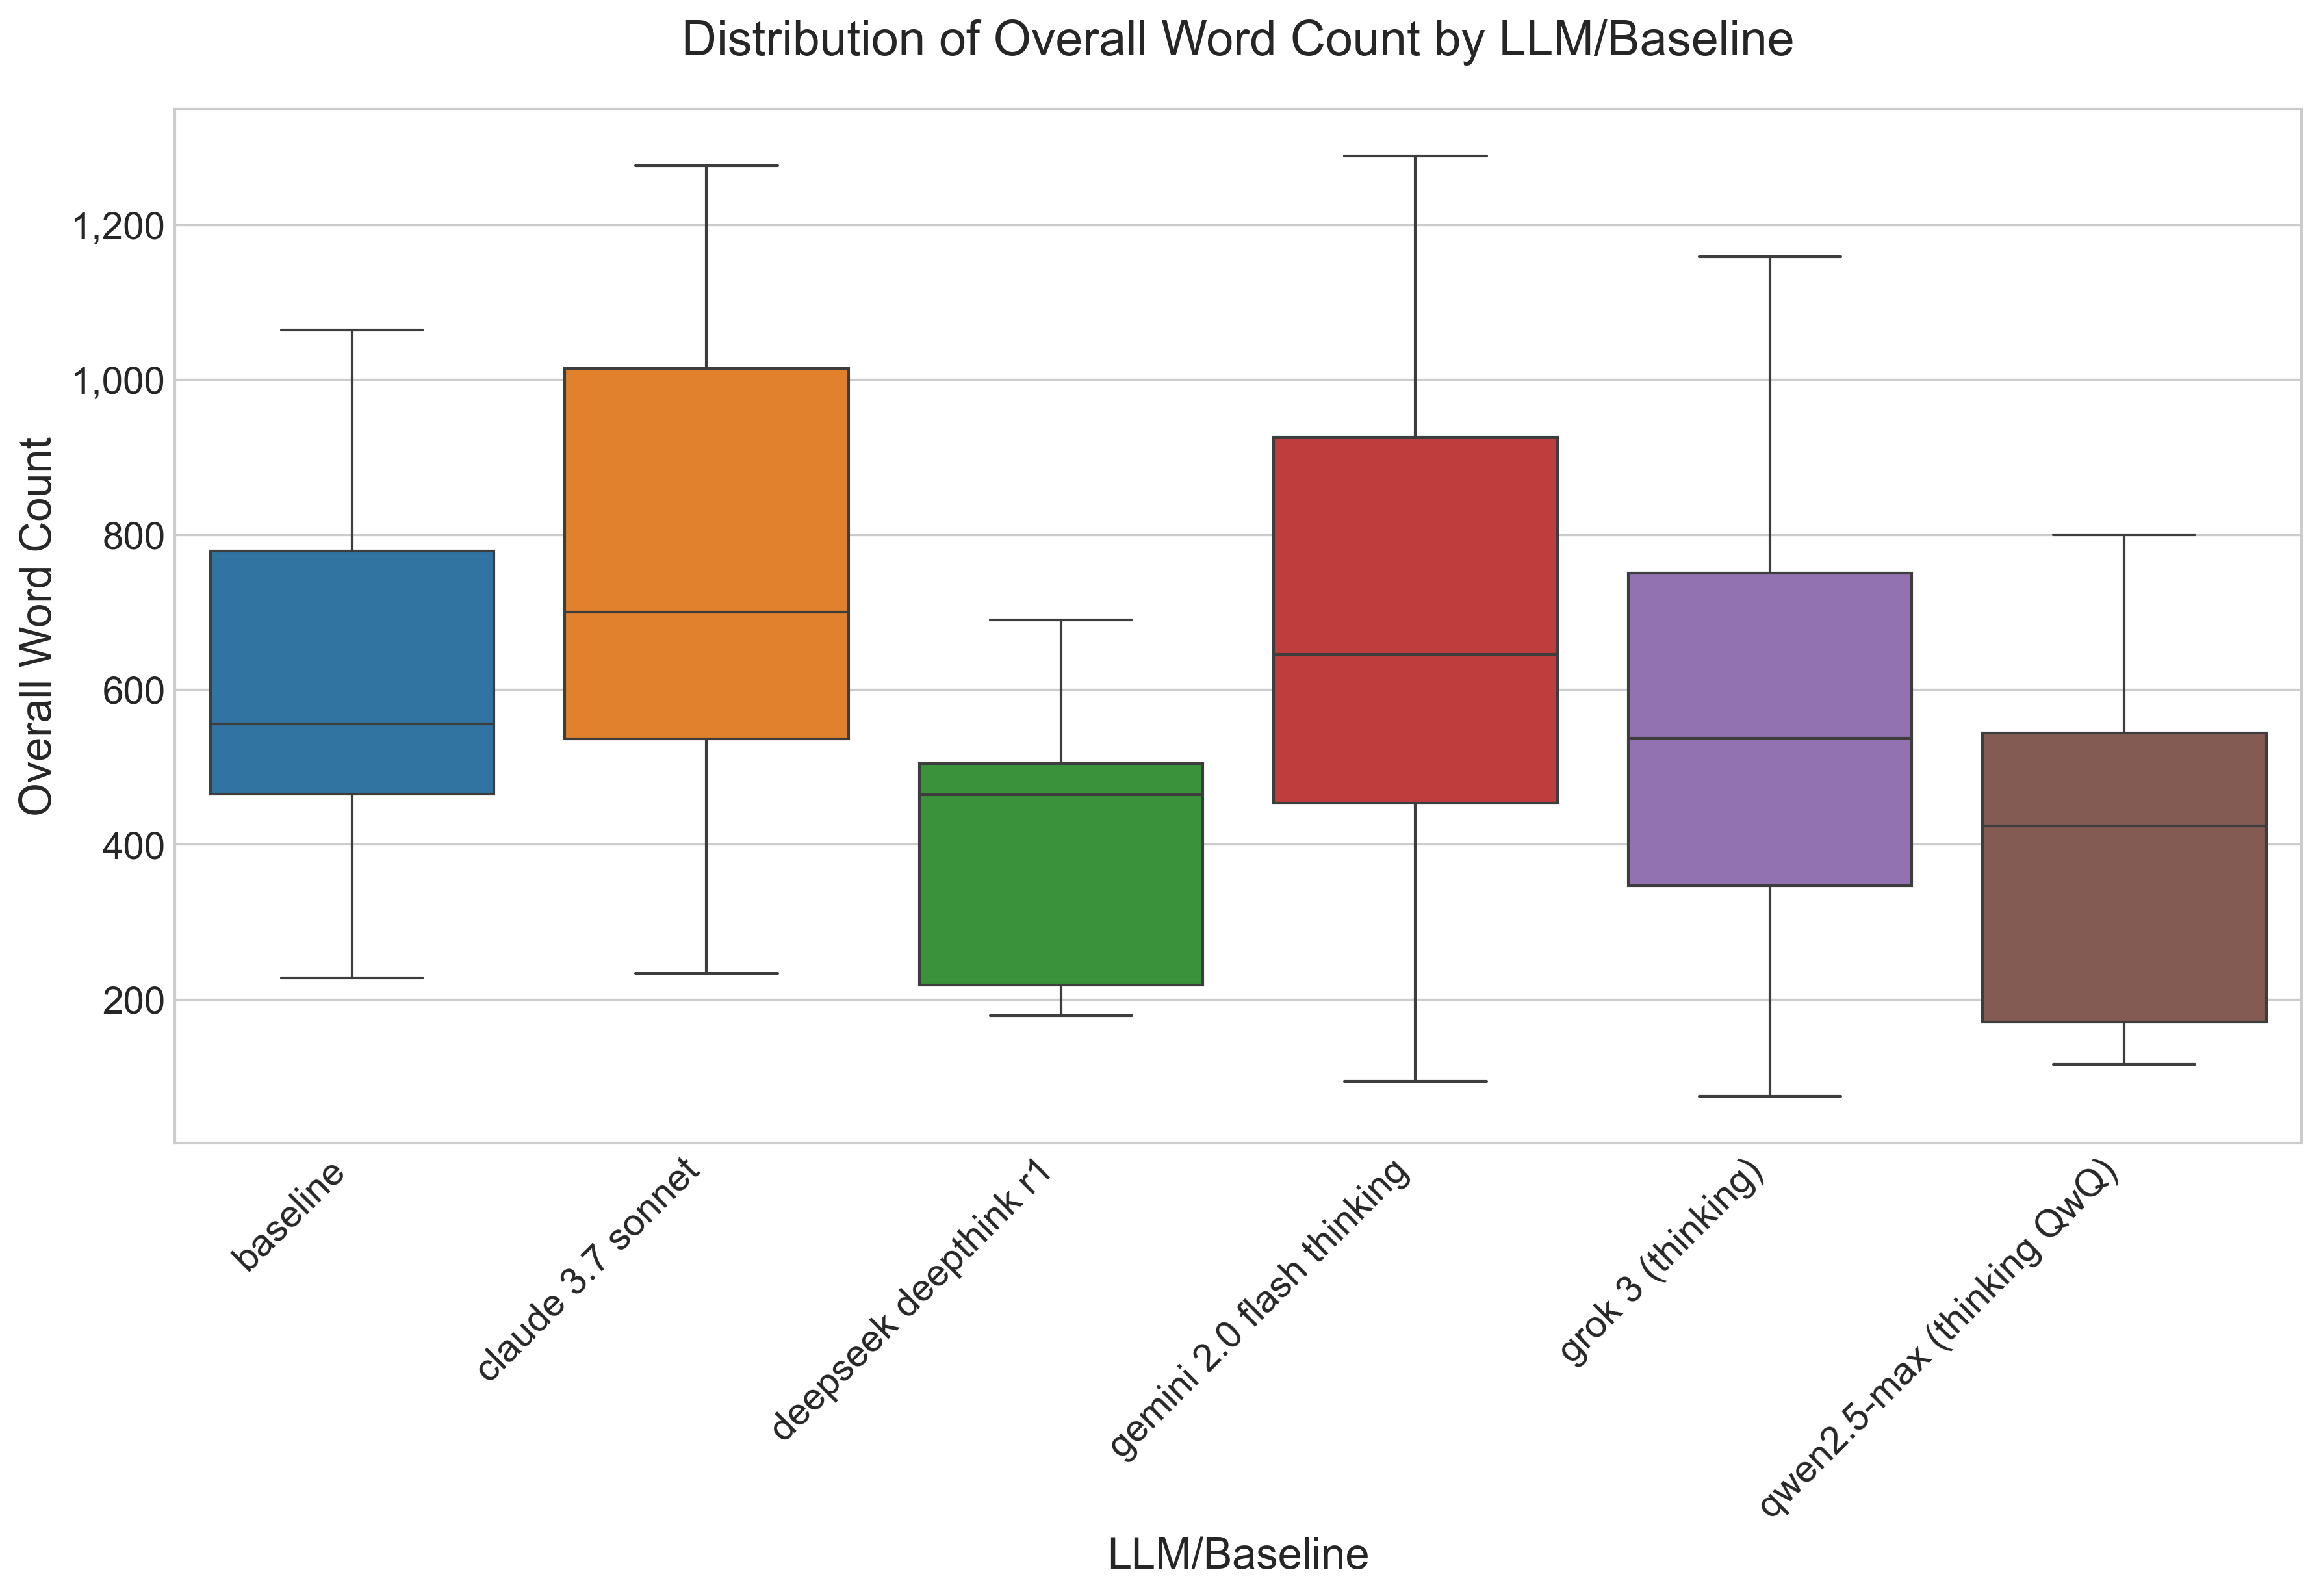
\includegraphics[width=0.8\linewidth]{evaluation/images/variability_by_llm_overall_word_count.png} % Replace with actual path
    \caption{Variability in Overall Word Count across LLMs (Avg D, ID, IO).}
    \label{fig:agnosticism_word_count_by_llm_igc_enriched}
\end{figure}

% Add table summarizing IO metric variability across models
\begin{table}[htbp]
\centering
\caption{Variability of Metrics for Improved Original (IO) Versions Across LLMs (Mean $\pm$ Std Dev over six PRs)}
\label{tab:agnosticism_metrics_summary}
\sisetup{round-mode=places, round-precision=1, table-format=4.1(3.1)} % Adjust format
\resizebox{\linewidth}{!}{%
\begin{tabular}{l S S S}
\toprule
LLM               & {Word Count (Total)} & {Flesch Ease (Body)} & {Sentiment (Comp.)} \\ % Use siunitx column types
\midrule
ChatGPT-4o (Base) & 767.5 \pm 320.0  & 6.3 \pm 27.5   & 0.7 \pm 0.5   \\
Claude 3.7 Sonnet & 1744.0 \pm 850.2 & 15.5 \pm 21.3  & 1.0 \pm 0.0   \\
Deepseek Deepthink& 421.8 \pm 197.1  & 12.1 \pm 18.7  & 0.9 \pm 0.2   \\
Gemini 2.0 Flash  & 573.0 \pm 214.5  & 16.0 \pm 19.6  & 0.9 \pm 0.1   \\
Grok 3            & 521.2 \pm 225.8  & 21.1 \pm 16.6  & 0.0 \pm 1.0   \\
Qwen2.5-Max       & 431.2 \pm 137.4  & 11.9 \pm 17.5  & 0.8 \pm 0.2   \\
\midrule
Overall Avg (IO)  & 743.1 \pm 547.0 & 13.8 \pm 21.1 & 0.7 \pm 0.6 \\ % Calculated overall avg for IO
\bottomrule
\end{tabular}%
}
\end{table}

\subsubsection{Similarity Analysis}
\begin{itemize}
    \item \textbf{Readability:} No significant difference in readability between the Original (O) versions and any of the generated versions (D, ID, IO). There was also no difference between the two improved versions (ID vs IO).
    \item \textbf{High Semantic Similarity:} Alternatives closely matched baseline meaning. The mean SBERT Cosine $\approx 0.735 \pm 0.202$, whereas the mean BERTScore F1 $\approx 0.845 \pm 0.028$, see (Fig. \ref{fig:agnosticism_sbert_by_llm_igc_enriched}).
    \item \textbf{Low Lexical Similarity:} Phrasing varied significantly. Mean BLEU $\approx 0.031 \pm 0.033$, while mean ROUGE-L F1 (body) $\approx 0.222 \pm 0.083$. There was a moderate term overlap (TF-IDF Cosine $\approx$ 0.5-0.6), see (Fig. \ref{fig:agnosticism_bleu_by_llm_igc_enriched}).
    \item \textbf{Sentiment Analysis:} The average sentiment scores were neutral to positive for both the IO (mean 0.730) and ID (mean 0.961) variants, likely due to their more formal or explanatory tone. Degraded (D) variant was more variable and slightly positive (mean 0.167) but spanning into negative territory. No model consistently generated more positive or negative sentiment across tasks.

\end{itemize}
These similarity measures partially suggest some level of model agnosticism, i.e., semantic intent transfers, but lexical realization does not.

\begin{figure}[htbp] % Existing Figure
    \centering
    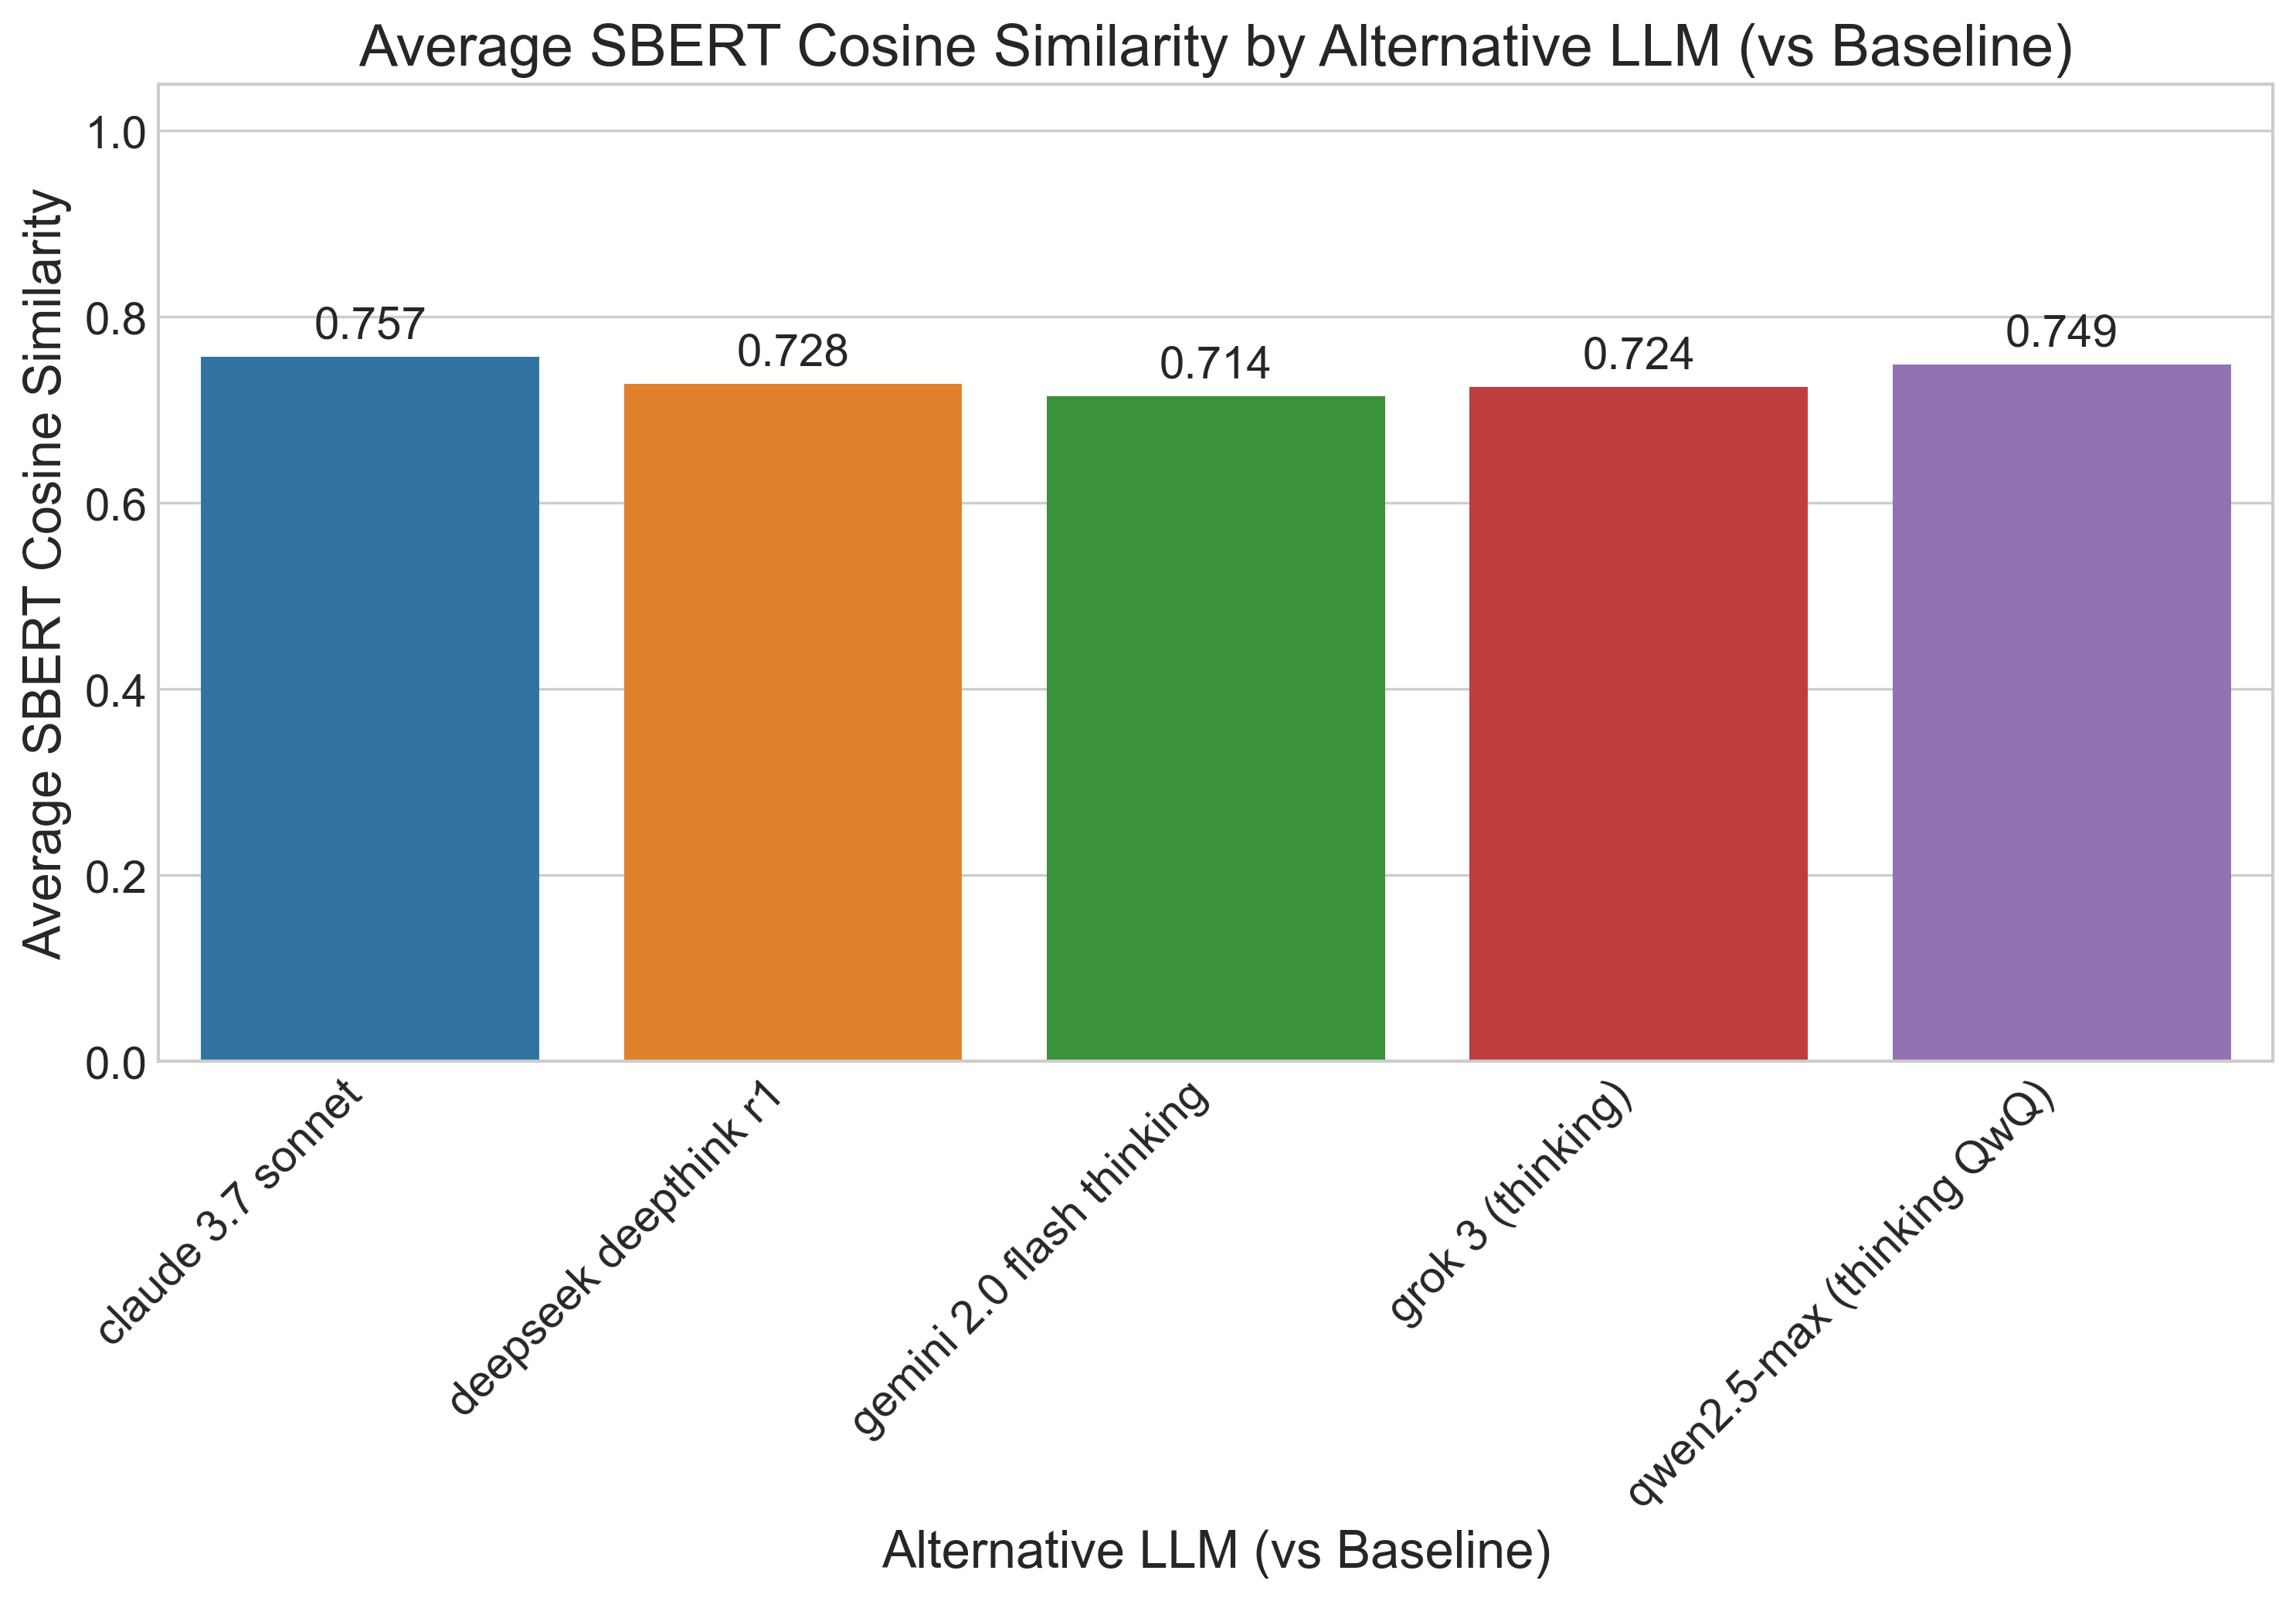
\includegraphics[width=0.8\linewidth]{evaluation/images/similarity_by_llm_sbert_cosine.png} % Replace with actual path
    \caption{High Semantic Similarity (SBERT Cosine) vs. Baseline.}
    \label{fig:agnosticism_sbert_by_llm_igc_enriched}
\end{figure}

\begin{figure}[htbp] % Existing Figure
    \centering
    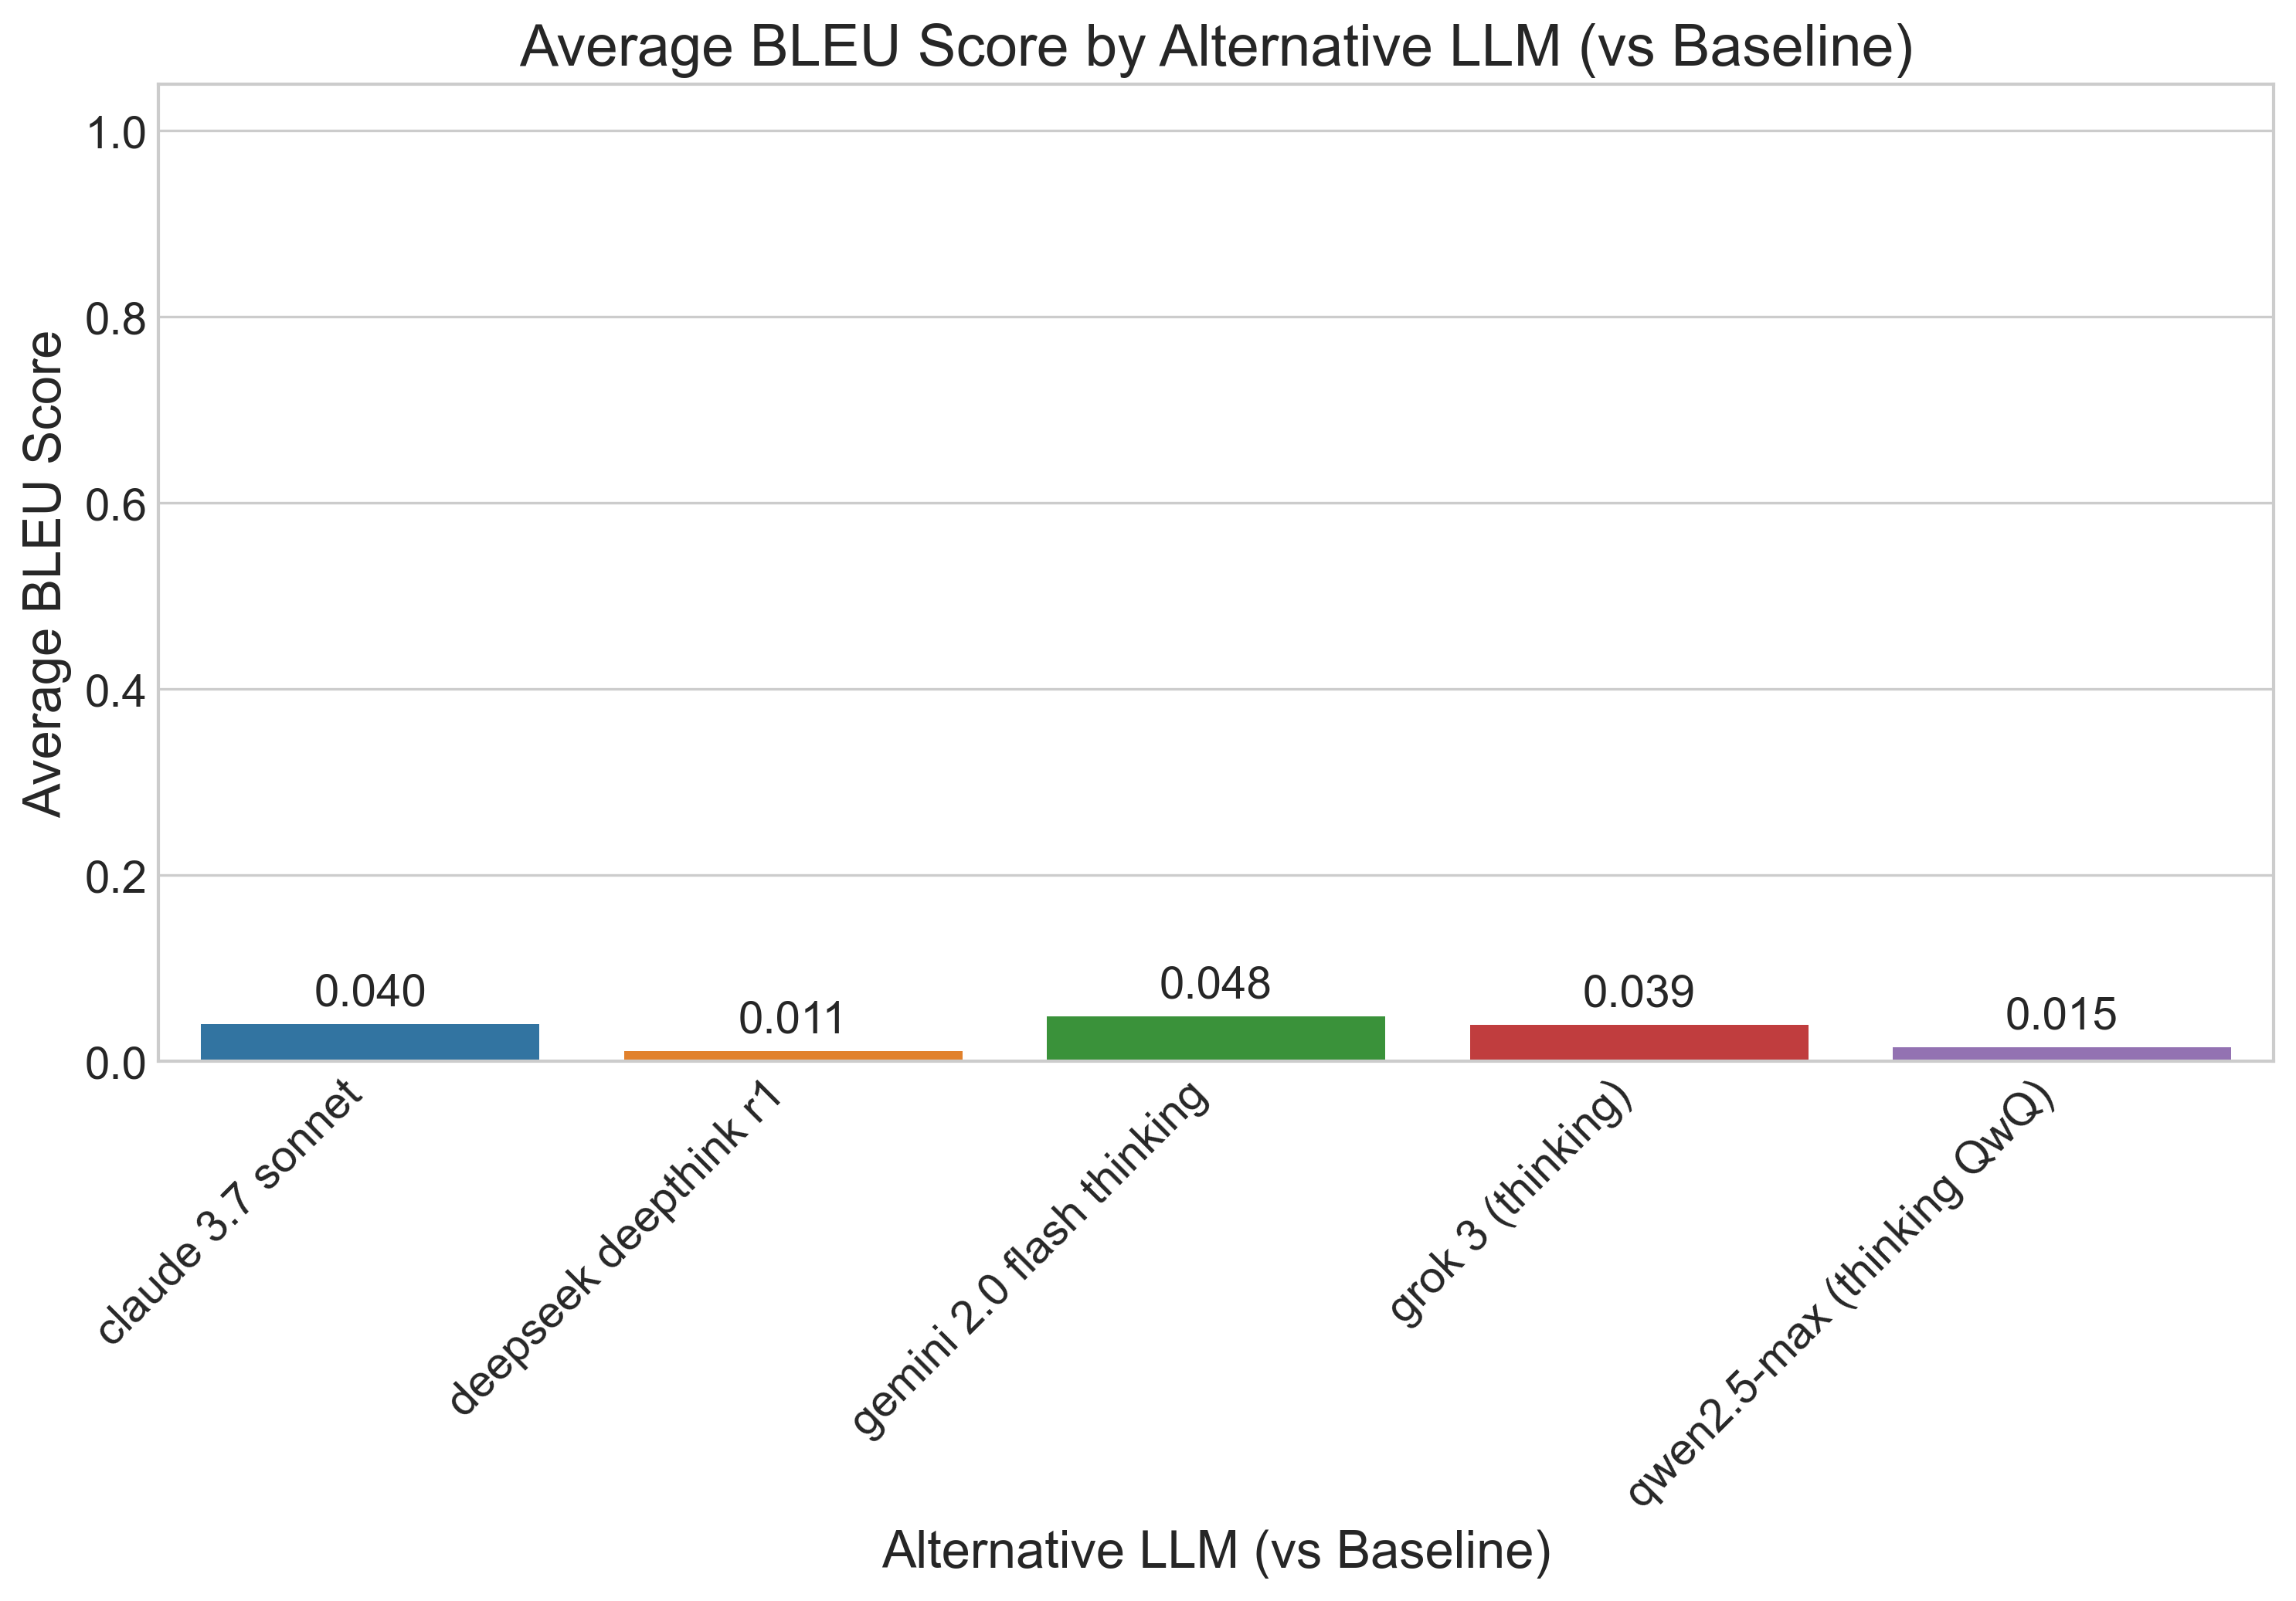
\includegraphics[width=0.8\linewidth]{evaluation/images/similarity_by_llm_bleu.png} % Replace with actual path
    \caption{Low Lexical Similarity (BLEU) vs. Baseline.}
    \label{fig:agnosticism_bleu_by_llm_igc_enriched}
\end{figure}

\section{Methodology for RQ3 and RQ4} % Retained enhanced methodology
Our approach involved selecting baseline PRs, generating variations, and evaluating them via a human survey.

\subsection{Baseline PR Selection and Variation Generation}
We first automatically scored 212k+ PRs from 82 repositories using ModernBERT \cite{warner2024smarter} based on six SE competencies \cite{wurzel2023competencies} adapted for PR text assessment (Architecture Impact, Code Quality, etc.). Six baseline Original (O) PRs were selected from high-scoring candidates after unanimous 'good' ratings from two experts.

Using ChatGPT-4o and specific prompts referencing these competencies, we generated three variations for each Original O PR: Degraded (D), Improved Original (IO), and Improved Degraded (ID).

\subsection{Survey Design and Execution}
A survey targeted software professionals (N=38; 71\% 5+ years experience; 71\% in developer role) recruited within Mercedes-Benz Tech Innovation GmbH, University of Postdam, and online. After consent and demographics, participants performed six tasks, each comparing two PR timelines side-by-side (Fig. \ref{fig:survey_comparison_example_erv_refined}) and choosing "Left", "Right", or "Neither" was better, with optional qualitative remarks (script \texttt{D6}).

\begin{figure}[htbp]
    \centering
    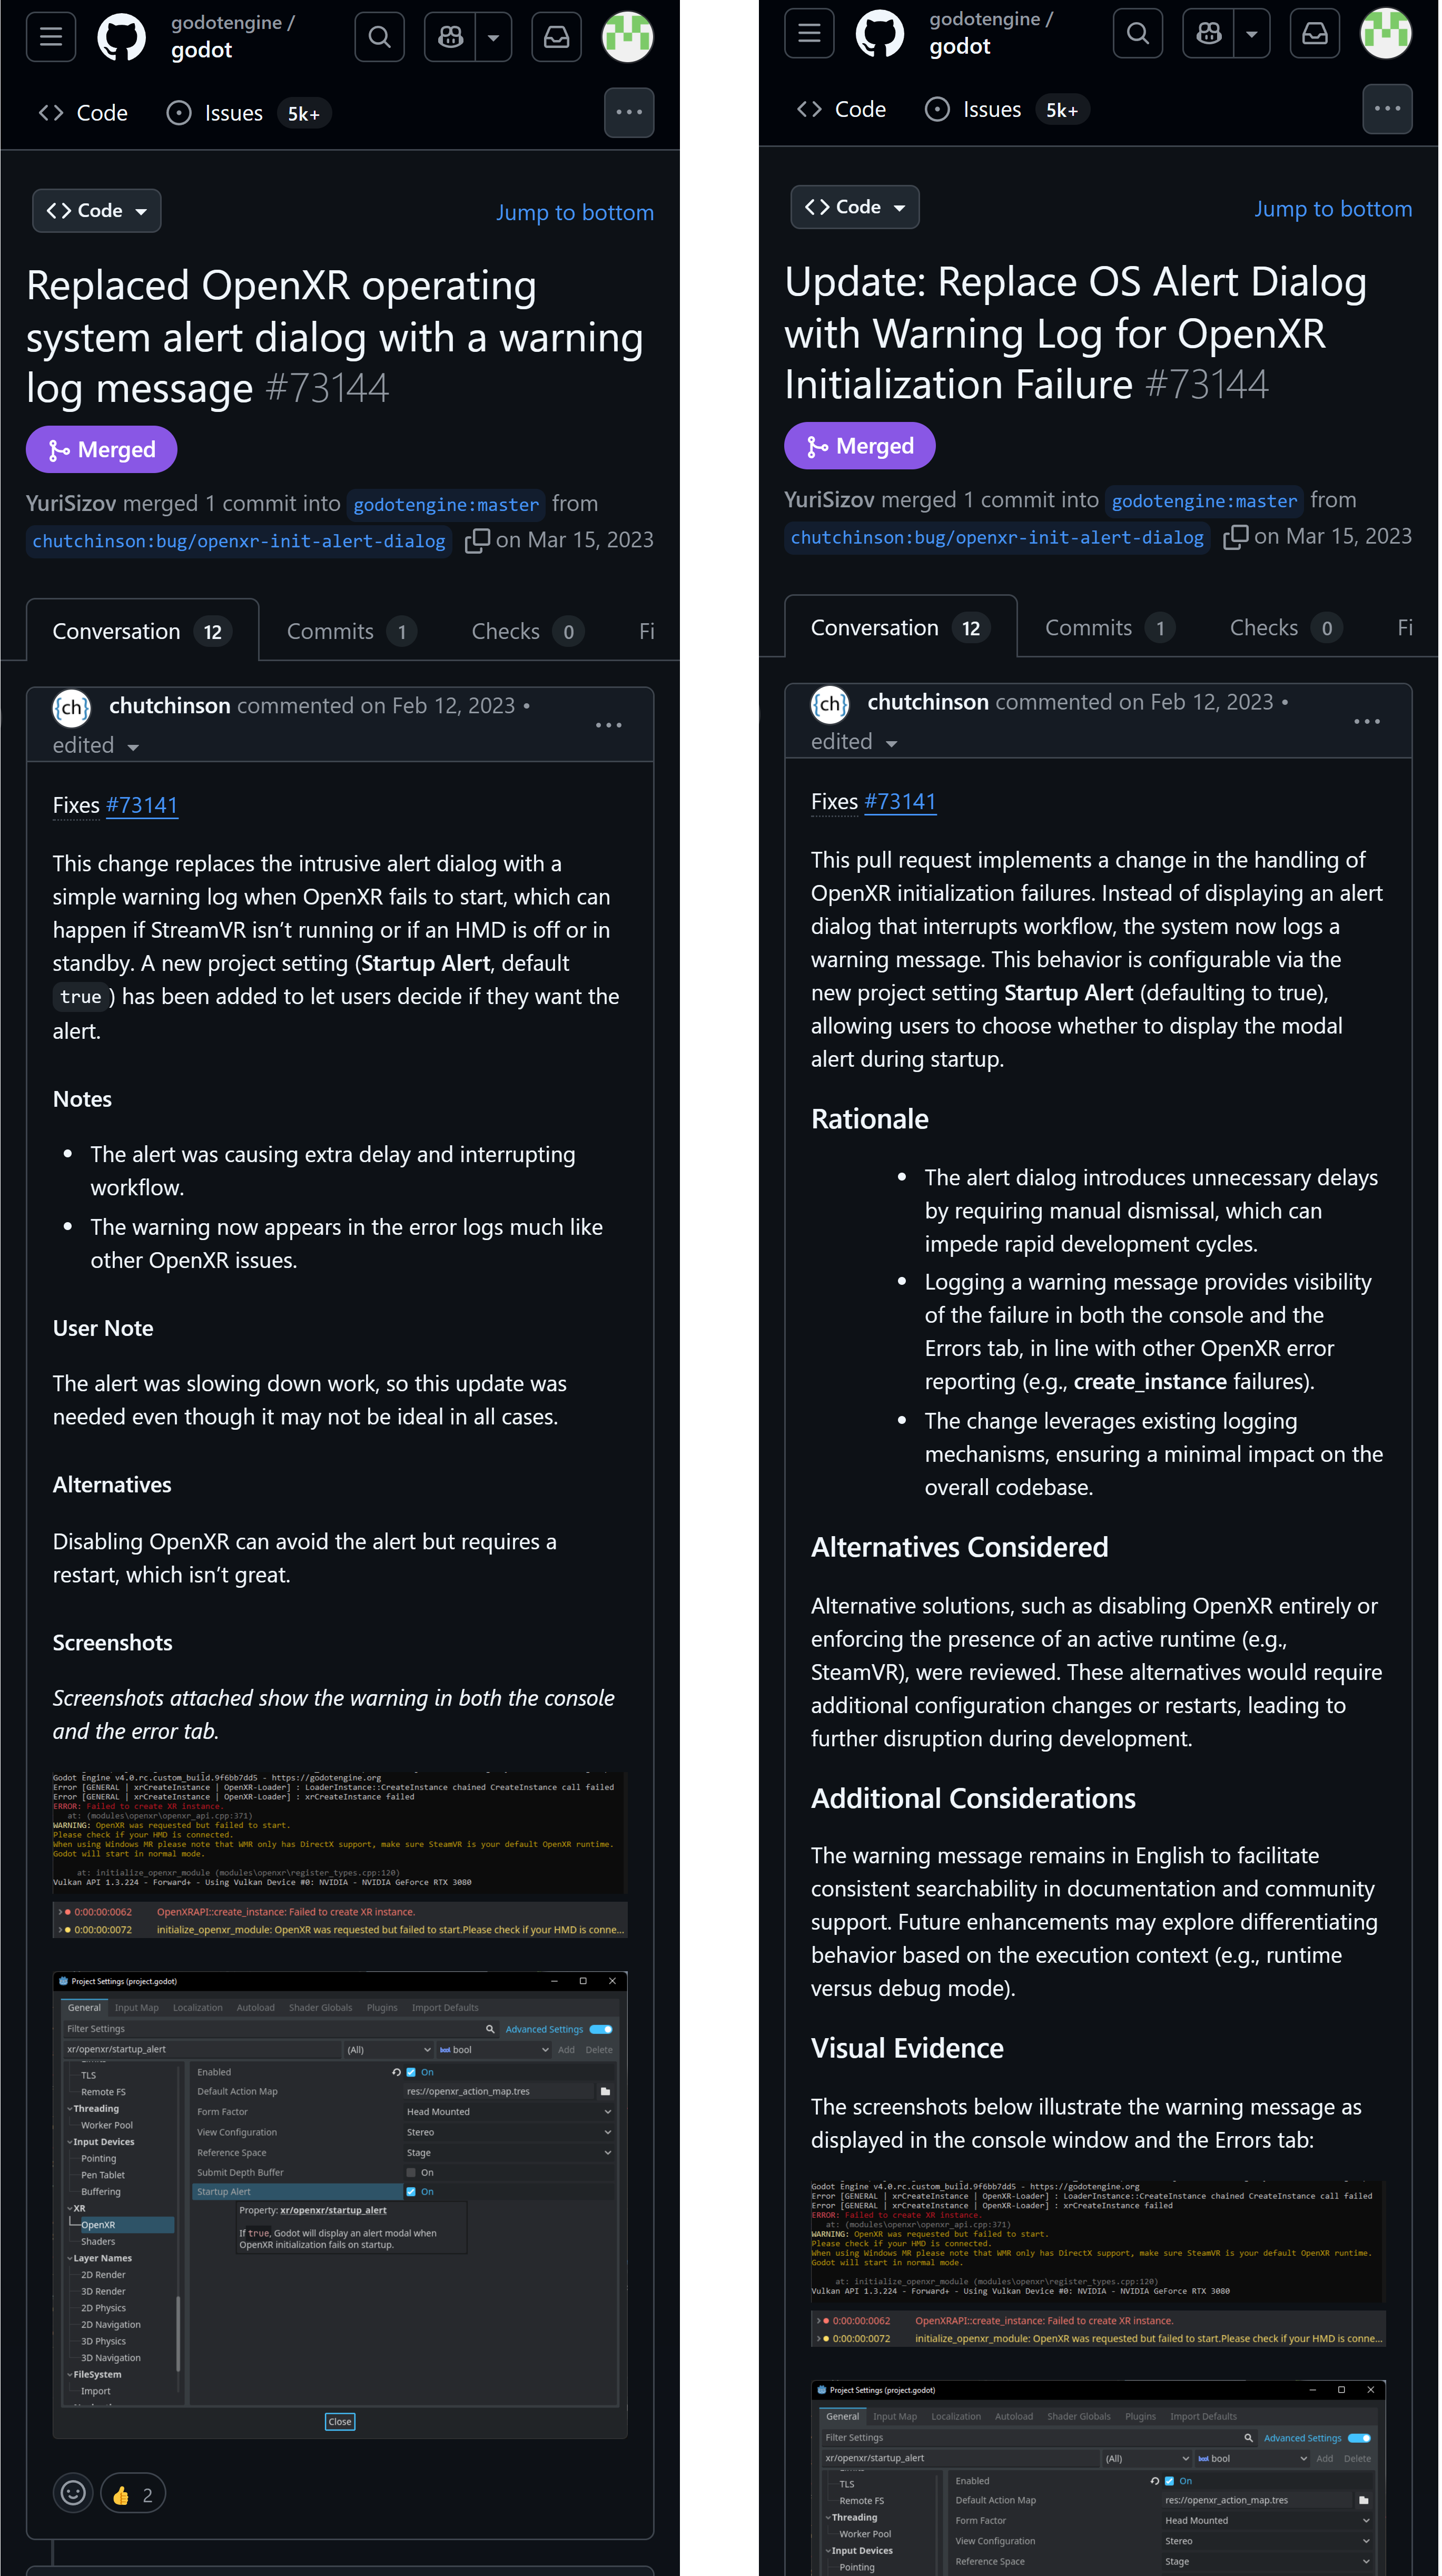
\includegraphics[width=\linewidth]{evaluation/images/PR_side-by-side.png}
    \caption{Degraded PR (left) and Original PR (right) placed automatically side-by-side by our tool.}
    \label{fig:survey_comparison_example_erv_refined}
\end{figure}

A $6 \times 6$ Latin Square design (script \texttt{D1}) balanced PR stimuli across comparison types and survey versions. A JavaScript load balancer randomly distributed participants among experimental conditions in a way that each condition progressed uniformly.

%(\texttt{S9}, Fig. \ref{fig:survey_load_balancer_flowchart_refined}) distributed participants.

%\begin{figure}[htbp]
%    \centering
%    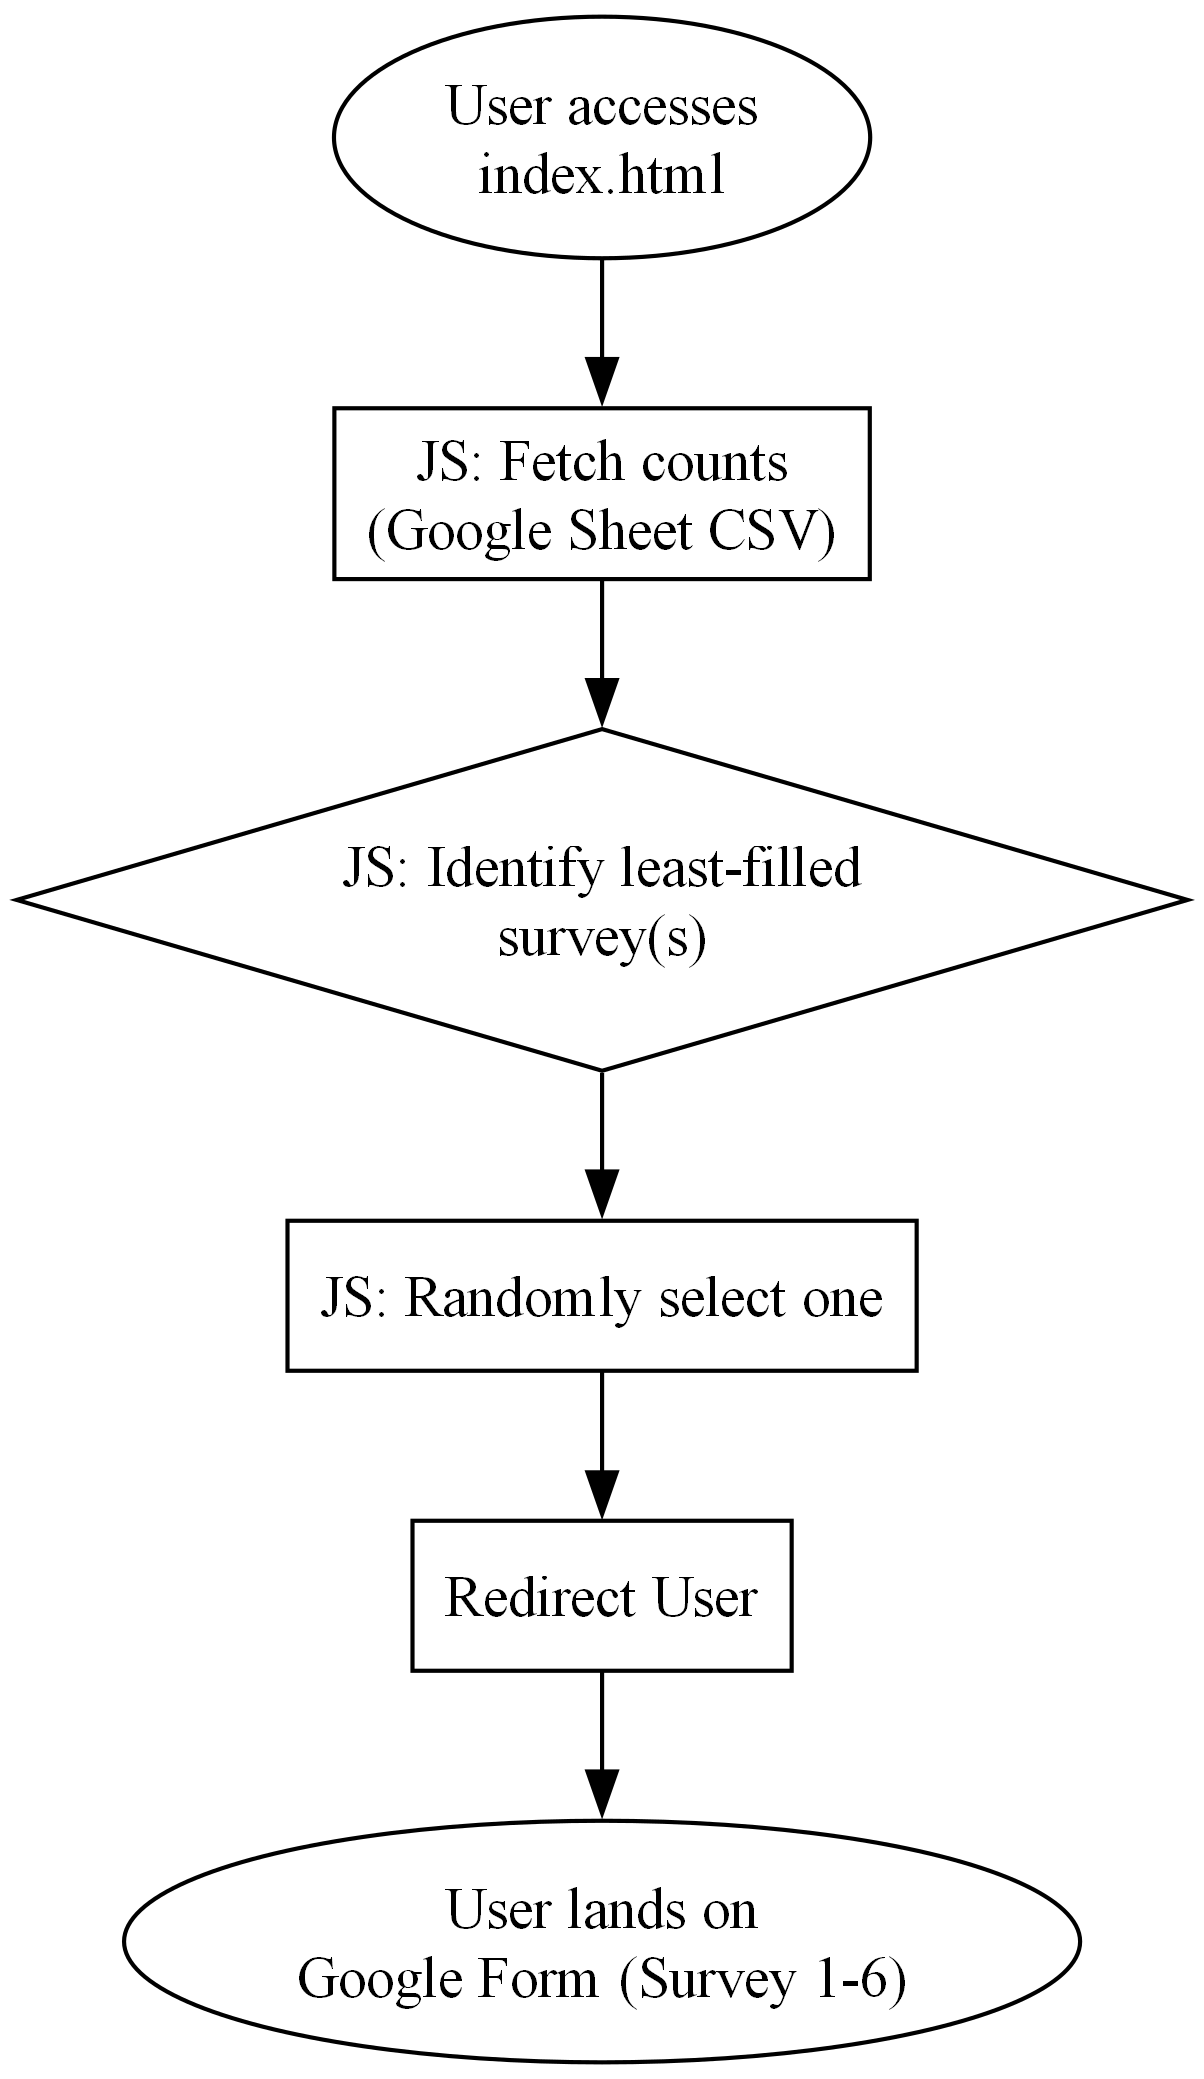
\includegraphics[width=0.8\linewidth]{evaluation/images/survey_load_balancer_flowchart.png} % Replace with actual path
 %   \caption{Survey Load Balancer Workflow.}
 %   \label{fig:survey_load_balancer_flowchart_refined}
%\end{figure}

\subsection{Data Analysis}
Quantitative preferences (excluding 'Neither') were analyzed using one-sided binomial tests ($\alpha=0.05$). Qualitative remarks (N=46) underwent thematic analysis. Our exploratory analyses did not found any significant demographic effects on developer's preferences.

\section{Answers to RQ3 and RQ4} % Retained enhanced results
\subsection{Quantitative Preferences}
Key binomial test results (Table \ref{tab:hypothesis_results_erv_refined}) revealed:
\begin{itemize}
    \item \textbf{ID significantly preferred over D (H3):} $p=0.029$.
    \item \textbf{ID significantly preferred over O (H5):} $p=0.026$.
    \item \textbf{No significant difference between O and D (H1/H7):} $p > 0.50$.
    \item \textbf{IO trends positive but not significant:} Preferences leaned towards IO over O (H2: $p=0.075$), ID (H4: $p=0.075$), and D (H6: $p=0.088$), with $\approx$63-65\% preference.
\end{itemize}

\begin{table}[htbp]
    \centering
    \caption{Key Binomial Hypothesis Test Results ($\alpha = 0.05$)}
    \label{tab:hypothesis_results_erv_refined}
    \sisetup{round-mode=places, round-precision=1}
    \begin{tabular}{l S[table-format=2.0] S[table-format=2.0] S[table-format=2.1] l c}
        \toprule
        Hypothesis & {N Winner} & {N Loser} & {\% Winner\textsuperscript{a}} & {$p$-value} & {Sig.} \\
        \midrule
        H1: $O > D$   & 15 & 16 & 48.4 & 0.640 & (ns) \\
        H7: $D > O$   & 16 & 15 & 51.6 & 0.500 & (ns) \\
        \textbf{H3: $ID > D$}  & \textbf{23} & \textbf{11} & \textbf{67.6} & \textbf{0.029} & * \\
        \textbf{H5: $ID > O$}  & \textbf{19} & \textbf{8}  & \textbf{70.4} & \textbf{0.026} & * \\
        H2: $IO > O$  & 20 & 11 & 64.5 & 0.075 & (ns) \\
        H4: $IO > ID$ & 20 & 11 & 64.5 & 0.075 & (ns) \\
        H6: $IO > D$  & 22 & 13 & 62.9 & 0.088 & (ns) \\
        \bottomrule
    \end{tabular}
    \textsuperscript{a}\% Winner calculated from (N Winner + N Loser). Total N=38 per comparison; 'Neither' choices ranged 10-29\%. * $p < 0.05$; (ns) $p \ge 0.05$. 
\end{table}

\subsection{Qualitative Insights} % Retained enhanced insights
Thematic analysis of 46 remarks from subject participants (indexed, for instance, S1\_P2) identified four key themes influencing their preference:
\begin{enumerate}
    \item \textbf{Detail vs. Conciseness:} A core subjective trade-off explaining O vs D ambiguity. Some preferred O's detail (subject S1\_P0), others D's brevity (subjects S1\_P1, S1\_P3).
    \item \textbf{Structure and Readability:} Added structure in ID/IO (summaries, checklists) was consistently valued for enhancing clarity (subject S1\_P3 on ID; S1\_P1 on IO), likely driving $ID > O$ significance.
    \item \textbf{Tone and Perceived Source:} Often negative for IO, criticized for "word noise," being "generic," "contrived," or "marketing material" (subjects S1\_P1, S1\_P3, S5\_P3). This artificiality likely undermined IO's benefits. O/ID sometimes preferred for feeling "human" (subjects S1\_P0, S1\_P3). Accuracy concerns about AI were also noted (subject S2\_P2).
    \item \textbf{Ambivalence/Minor Differences:} Frequent "Neither" choices due to perceived parity or balanced trade-offs (subject S1\_P1).
\end{enumerate}

The results show that LLMs can generate PR descriptions that are perceived to be superior to human-generated ones (ID $>$ O). The reason seems to be the ability of LLMs to enrich the original content with structure. This supports using LLMs to enhance poor descriptions or apply structural best practices.

However, the IO results highlight critical limitations. Adverse reactions to tone/verbosity suggest naive "improvement" prompts can trigger homogenization effects \cite{lee2025poor}, producing unnatural text disliked by users. This aligns with controllability challenges \cite{lee2025poor, yang2024survey} and expert skepticism about AI replicating subjective judgment. Practical AI assistance likely requires targeted prompting or better stylistic control. The O vs D ambiguity confirms the subjectivity of developers' information needs \cite{bacchelli2013expectations}.

%------------------------------------
\section{Discussion: Implications to Industry and Bridging Results to the Software Practice} \label{sec:implications}

\subsection{Implications of Automated Scoring for Industry}
The automated scoring approach shows potential for large-scale monitoring of PR quality dimensions across projects or business units. Identifying repository archetypes based on competency profiles (e.g., Cluster 0 strong on impact, Cluster 1 on collaboration, Cluster 2 on maintainability) could help organizations understand team strengths or tailor process improvements. Tracking scores over time might surface process changes or team composition trends. However, direct use requires caution: the underlying classifier needs validation, especially on proprietary code, and scores should complement, not replace, human judgment.

\subsection{Implications of Partial Model Agnosticism for Industry}
Our finding of partial model agnosticism – consistent semantics but variable style – is critical for industrial LLM deployment for at least three reasons:
\begin{itemize}
    \item \textbf{User Experience \& Training:} Significant variation in length (Table \ref{tab:agnosticism_metrics_summary}) and readability means UX can change drastically if LLM back-ends are swapped. User acceptance might depend heavily on the chosen model's default style (e.g., avoiding excessive verbosity).
    \item \textbf{Cost and Performance:} The larger than 4 times difference in average IO length directly impacts API costs and processing time. Selecting a more concise model (like Deepseek or Qwen in our tests) could yield substantial savings over a more verbose one (like Claude Sonnet) for the same semantic task.
    \item \textbf{Tool Selection \& Consistency:} Relying on LLMs requires acknowledging this variability. Teams must choose a model whose style aligns with their needs, invest in model-specific prompt engineering/tuning, or build flexible tools to handle different LLM outputs. Simply assuming functional equivalence is insufficient for predictable industrial tools.
\end{itemize}
Model awareness is therefore essential for managing costs, ensuring consistent UX, and maintaining tool stability in production environments.

\subsection{Bridging Research to Practice: A Prototype Feedback System}
We developed a prototype system at the Mercedes-Benz Tech Innovation GmbH to translate these findings into practice. This prototype delivered a personalized, competency-based feedback nudges on closed PRs.
\begin{itemize}
    \item \textbf{Rationale:} It addresses the need for customization (developers select competencies) and model flexibility (supports multiple LLM back-ends) highlighted by our findings. Focusing on specific competencies and PR context aims for targeted feedback, potentially avoiding basic mistakes.
    \item \textbf{Integration:} It integrates directly into the GitHub workflow via the `pull\_request.closed` event, fetching metadata, constructing dynamic prompts, querying a configured LLM, and delivering personalized nudges to contributors.
    \item \textbf{Industrial Value Proposition:} This approach demonstrates how LLMs can be used for targeted developer support and learning within existing workflows, potentially improving specific skill areas identified via scoring or team goals, while accounting for model differences.
\end{itemize}
This prototype is a concrete example of applying empirical insights on competency scoring and model variability to design practical, industry-relevant AI assistance.

\subsection{Perspectives on Code Review Assistance} % Enhanced Vision/Future Work
Our results support a vision where AI assists code review by handling objective tasks while humans retain control over subjective elements. We envision AI tools that:
\begin{itemize}
    \item \textbf{Focus AI on Strengths:} Leverage LLMs primarily for objective enhancements like generating summaries, extracting key changes, creating checklists based on requirements, or ensuring adherence to structural templates – tasks where our results show clear value (e.g., the ID version).
    \item \textbf{Enable Controllable Generation:} Develop mechanisms beyond simple prompts to allow users fine-grained control over output style, verbosity, and tone. This might involve interactive refinement, style parameters, or model fine-tuning targeted at specific stylistic goals, directly addressing the shortcomings observed with the IO version.
    \item \textbf{Facilitate Human-AI Collaboration:} Design interfaces where AI suggestions (especially stylistic ones) are presented as options or nudges \cite{caraban2019ways}, allowing developers to easily accept, reject, or modify them, thus maintaining human agency and mitigating risks of over-reliance or adoption of suboptimal AI outputs \cite{gao2023impact}.
    \item \textbf{Support Personalization:} Explore adaptive systems that learn individual or team preferences regarding information density and communication style \cite{zhang2024personalization}, moving beyond one-size-fits-all solutions.
    \item \textbf{Require Robust Evaluation:} Future work must rigorously evaluate such tools in diverse, realistic contexts (in-situ studies, varied projects) \cite{robillard2024communicating}, assessing not just technical performance but also user acceptance, trust \cite{mehrotra2024systematic}, and impact on review effectiveness and team dynamics.
\end{itemize}
Addressing fundamental LLM controllability challenges \cite{lee2025poor} and understanding model agnosticism remain crucial research avenues. Our proof-of-concept system providing personalized, competency-based feedback via a GitHub Action represents an initial step towards realizing parts of this vision, focusing on targeted nudging rather than broad text generation.

\section{Limitations and Threats to Validity}
\label{sec:discussion_limitations}

While we followed the best practices in empirical software engineering methodology\cite{ko2015practical,wieringa2014design
}, our study still presents several limitations and potential threats to validity~\cite{wohlin2012experimentation,siegmund2015views} that must be acknowledged.

\subsection{Limitations}

\textbf{Sample Size and Representativeness} -- The survey involved 38 participants. While primarily experienced professionals, they may not represent the full diversity of the global software engineering population. Recruitment was opportunistic, potentially introducing selection bias. The qualitative analysis is based on 46 remarks, offering depth but limited breadth.

\textbf{Stimuli Specificity} -- The study used six baseline PRs selected from open-source projects. Findings might not generalize to PRs from different domains, sizes, complexities, or proprietary code bases. The specific LLM used for survey stimuli (ChatGPT-4o) and the other five used for agnosticism testing represent only a fraction of the available models.

\textbf{Focus on Descriptions Only} -- The evaluation focused solely on the PR description timeline (title, body, comments). It did not involve evaluating the code changes, which is a critical part of an honest code review. Perceptions might differ when descriptions are viewed alongside code.

\textbf{Artificial Survey Setting} -- Participants evaluated static images of PR timelines in a controlled survey environment, differing from the dynamic context of actual code review tools and workflows. The side-by-side comparison format might encourage more critical scrutiny than usual. Potential order effects were mitigated by the Latin Square design, but cannot be entirely ruled out.

\textbf{LLM Interaction Nuances} -- The study used specific prompts and settings (e.g., reasoning mode). Different prompting strategies or LLM configurations could yield different results, although the referenced work suggests simple demographic prompting is generally ineffective for alignment \cite{lee2025poor}. The 'Degraded' version was created artificially; naturally occurring low-quality PRs might differ.

\textbf{Subjectivity of Quality} -- The quality of a PR description is inherently subjective. While the study captured preferences, these reflect the aggregated views of this participant group and may not represent universal optima.

\textbf{Prototype Description Scope} -- The prototypical GitHub Action described alongside this research is provided at a high level. Specific implementation details and prompt engineering techniques may be subject to confidentiality constraints of the collaborating industrial partner (Mercedes-Benz Tech Innovation GmbH). 

\subsection{Threats to Validity}

\textbf{Internal Validity} -- Did the variations (D, ID, IO) cause the observed preferences? The controlled generation and Latin Square design help mitigate confounding factors related to specific PRs or presentation order. However, individual participant differences (experience, LLM familiarity, personal preferences) remain a source of variance, as acknowledged by the lack of significant demographic correlations in our initial exploratory analysis.

\textbf{Construct Validity} -- Does the survey measure the intended construct of "perceived quality"? The direct preference question ("Which was better?") relies on the participants' subjective interpretations of "better". The competencies used for generation guided the modifications, but were not explicitly measured in the perception phase. The automated scoring used for pre-filtering relies on the validity of the zero-shot classifier for those competencies. The qualitative remarks help triangulate the construct by revealing the reasons behind choices.

\textbf{External Validity (Generalizability)} -- Can the findings be generalized beyond this specific sample, stimuli, and LLMs? As discussed in the limitations, the sample characteristics constrain generalizability, the specific PRs chosen, and the limited set of LLMs evaluated. The partial model agnosticism finding addresses this, indicating that generalization requires caution regarding stylistic aspects. The alignment issues highlighted by Lee et al. \cite{lee2025poor} in a different domain (essays) suggest these controllability challenges might be widespread.

\textbf{Conclusion Validity} -- Are the statistical conclusions sound? One-sided binomial tests were used, which were appropriate for the directional hypotheses. The significance level was standard ($\alpha=0.05$). The interpretation acknowledges non-significant trends and relies on qualitative data to understand nuanced results, reducing the risk of overstating conclusions based solely on p-values. The exploratory demographic analyses were explicitly noted as such, mitigating the risk of Type I errors from multiple comparisons.

\section{Conclusion \& Future Work}\label{sec:conclusion}
This study demonstrated the potential of competency-based scoring for large-scale PR quality monitoring and revealed distinct project profiles. The evaluation of six state-of-the-art LLMs showed partial model agnosticism - semantic meaning was preserved. However, stylistic aspects such as length and readability varied, underscoring the need to select PR training examples in the industrial setting carefully. Developers valued the added structure in LLM-improved PR descriptions, but excessive verbosity and an "AI tone" sometimes produced unnatural, homogenized outputs that could limit adoption.

 Future work should validate our scoring approach in industrial settings, extending it to proprietary code-bases and diverse PRs across sizes, complexities, and domains, with a larger and more varied participant pool to improve generalizability. Advancing stylistic control across LLMs—through prompt steering, context engineering, and alignment with the company's code review culture~\cite{roychoudhury2025agentic} will be key to producing consistent, context-appropriate PRs. Novel human-centered AI methods should focus on adding structure to human-written PR descriptions,  while giving developers control over subjective style adjustments. One idea is to integrate description evaluation with the corresponding code changes to ensure that outputs are well-structured, accurate, and concise. Finally, exploring Agentic AI in PR and code review workflows~\cite{li2025rise} could illuminate how AI affects human collaboration and the socio-technical dynamics of the software development process.

\section*{Author Contributions}
\textbf{Luca Mariotto} developed the research during his internship at Mercedes-Benz Tech Innovation. He designed the methodology, conducted the experiments, performed the analyses, created all visualizations, and co-wrote the manuscript. \textbf{Christian M. Adriano}, Luca's academic supervisor, guided the experimental design and co-wrote the manuscript. \textbf{René Eichhorn}, the industry supervisor, provided access to data and infrastructure, facilitated contact with Mercedes-Benz Tech Innovation study participants, and reviewed the manuscript. \textbf{Daniel Burgstahler} and \textbf{Holger Giese} contributed to the project conception and resources, and reviewed the results.

\section*{Acknowledgment}
We thank the support of Mercedes-Benz Tech Innovation GmbH and the Hasso Plattner Institut for Digital Engineering gGmbH. We are particularly grateful to the 38 anonymous developers who participated in the experiments.

\bibliographystyle{IEEEtran}
\bibliography{IEEEabrv, references_paper} % Ensure 'references.bib' exists

\end{document}